\documentclass[9pt,pdftex,aspectratio=1610]{beamer}
\usepackage{amsmath, amsthm, amssymb}
\usepackage{color}
\usepackage{hyperref}
\usepackage{subfigure}
\usepackage{tabularx}
\usepackage{ragged2e}
\usepackage{booktabs}
\usepackage{multirow}
\usepackage{natbib}
\usepackage{bbm}

\usecolortheme{dolphin}
\linespread{1.3}
\definecolor{nblue}{RGB}{0,0,128}

\bibliographystyle{ecta}
\setbeamercovered{transparent}

\newcolumntype{Y}{>{\RaggedRight\arraybackslash}X}
%\setbeamerfont{alerted text}{series=\bfseries}

\hypersetup{colorlinks=true, linkcolor=nblue,
citecolor=nblue, urlcolor=nblue, bookmarks=false,
pdfpagemode=UseNone,
pdfstartview={XYZ null null 1.0},
pdftitle={Heterogeneous Agent Trade},
pdfauthor={ Michael E. Waugh},
pdfkeywords={economics, trade, dynamics, quant econ, consumption, data science,
waugh, incomplete markets, inequality, Ricardo, julia, Armington, China, trade war, tariffs, python, matplotlib}}

%\usepackage[pdftex,colorlinks=true, bookmarks=false,
%pdfstartview={XYZ null null 1.0},
%pdftitle={Heterogeneous Agent Trade},
%pdfauthor={Michael E. Waugh},
%pdfkeywords={economics, trade, dynamics, quant econ, consumption, data science,
%waugh, incomplete markets, inequality, Ricardo, julia, Armington, China, trade war, tariffs, python, matplotlib},
%colorlinks=true,linkcolor=darkgray,citecolor=darkgray,urlcolor=darkgray,
%breaklinks]{hyperref}

\setbeamertemplate{navigation symbols}{}
\setbeamertemplate{footline}[frame number]
\setbeamertemplate{theorems}[numbered]
\setbeamertemplate{itemize subitem}[circle]
\setbeamertemplate{enumerate items}[default]

\setbeamerfont{frametitle}{size= \large}
\setbeamerfont{ framesubtitle }{size = \footnotesize}
\setbeamertemplate{frametitle}
{
\medskip
\smallskip
{\textsf{\underline{\insertframetitle\phantom{))))))))}}}}}
\setbeamertemplate{items}[circle]
\setbeamertemplate{itemize subitem}[circle]

\theoremstyle{definition}


\newtheorem{as}{Assumption}
\newtheorem{df}{Definition}
\newtheorem{lm}{Lemma}
\newtheorem{prp}{Proposition}

\usepackage[normalem]{ulem}
\newcommand\redout{\bgroup\markoverwith
{\textcolor{red}{\rule[.5ex]{1pt}{1pt}}}\ULon}

\makeatletter
\def\blfootnote{\xdef\@thefnmark{}\@footnotetext}
\makeatother

%%%%%%%%%%%%%%%%%%%%%%%%%%%%%%%%%%%%%%%%%%%%%%%%%%%%%%%%%%%%%%%%%%%%%%%%%%%%%%%%%%%%%%%%%%%%%%%%%
%%%%%%%%%%%%%%%%%%%%%%%%%%%%%%%%%%%%%%%%%%%%%%%%%%%%%%%%%%%%%%%%%%%%%%%%%%%%%%%%%%%%%%%%%%%%%%%%%

%%%%%%%%%%%%%%%%%%%%%%%%%%%%%%%%%%%%%%%%%%%%%%%%%%%%%%%%%%%%%%%%%%%%%%%%%%%%%%%%%%%%%%%%%%%%%%%%%
%%%%%%%%%%%%%%%%%%%%%%%%%%%%%%%%%%%%%%%%%%%%%%%%%%%%%%%%%%%%%%%%%%%%%%%%%%%%%%%%%%%%%%%%%%%%%%%%%

\title{\Large Heterogeneous Agent Trade}
\institute[Foo and Bar]{\normalsize\begin{tabular}[h]{c}
Michael E. Waugh  \\
Federal Reserve Bank of Minneapolis\blfootnote{The views expressed herein are those of the author and not necessarily those of the Federal
Reserve Bank of Minneapolis or the Federal Reserve System. This project was developed with research support from the National Science Foundation (NSF Award number 1948800). Thomas Hasenzagl provided excellent research assistance.} and NBER\\
\href{https://twitter.com/tradewartracker}{@tradewartracker}
\end{tabular}}

\date{\today}

\begin{document}

\begin{frame}
\titlepage
\setcounter{framenumber}{0}
\section{}
\end{frame}

\begin{frame}[t]{What am I doing?}
\smallskip
To trade economists, household heterogeneity is interesting because of the notion that some benefit from trade and others don't.\\
\bigskip
One mechanism behind this notion is heterogeneity in \begin{alert}{\textbf{elasticities}}\end{alert}.
\begin{itemize}
\smallskip
\item \citet*{auer2022unequal} is a nice example. In the context of the 2015 Swiss appreciation, they find that poor households are more price elastic.
\end{itemize}
\bigskip
\medskip
This paper:\\
\begin{itemize}
\smallskip
\item A model of household heterogeneity in price elasticities at the micro level \emph{and} they arise because of a market failure, i.e., the lack of insurance against life's circumstances.\\
\medskip
\item And I use it as a laboratory to think about aggregate trade, the gains from trade and how they are distributed, and the normative implications, e.g., what \emph{should} the pattern of trade look like.
\end{itemize}
\end{frame}

%%%%%%%%%%%%%%%%%%%%%%%%%%%%%%%%%%%%%%%%%%%%%%%%%%%%%%%%%%%%%%%%%%%%%%%%%%%%%%%%%%%%%%%%%%%%%%%%%
%%%%%%%%%%%%%%%%%%%%%%%%%%%%%%%%%%%%%%%%%%%%%%%%%%%%%%%%%%%%%%%%%%%%%%%%%%%%%%%%%%%%%%%%%%%%%%%%%

\begin{frame}[t]{How I do it\ldots}
Two ingredients:
\begin{itemize}
\smallskip
\item Trade as in Armington, but households have random utility over varieties | \citet{mcfadden1974frontiers}
\smallskip
\item Standard incomplete markets model with households facing incomplete insurance against idiosyncratic productivity and taste shocks | \citet{bewley1979optimum}
\end{itemize}
\bigskip
\only<1>{
Qualitatively I characterize:
\begin{itemize}
\smallskip
\item How price elasticities vary at the micro-level and when micro-heterogeneity shapes aggregates.
\smallskip
\item The welfare gains from trade at the micro and macro level.
\smallskip
\item The efficient allocation and, thus, how market incompleteness shapes these outcomes.
\end{itemize}}
\only<2>{Quantitatively:
\begin{itemize}
\smallskip
\item I work at a scale typically reserved for static frameworks|I calibrate a 19 country model (the \citet{eaton2002technology} data set) to match trade flow data using ``gravity as a guide.''
\smallskip
\item Illustrate some workings of the model through gains from trade type calculations.
\smallskip
\item Compare trade in the efficient allocation vs. the decentralized allocation.
\end{itemize}}

\end{frame}

%%%%%%%%%%%%%%%%%%%%%%%%%%%%%%%%%%%%%%%%%%%%%%%%%%%%%%%%%%%%%%%%%%%%%%%%%%%%%%%%%%%%%%%%%%%%%%%%%
%%%%%%%%%%%%%%%%%%%%%%%%%%%%%%%%%%%%%%%%%%%%%%%%%%%%%%%%%%%%%%%%%%%%%%%%%%%%%%%%%%%%%%%%%%%%%%%%%

\begin{frame}[t]{Model: Production and Trade}
\smallskip
$M$ countries. Each country produces a nationally differentiated product as in Armington.\\
\bigskip
\medskip
In country $i$, competitive firms' produce variety $i$ with:
\begin{align*}
Q_i = A_i N_i,
\end{align*}
where $A_i$ is TFP; $N_i$ are efficiency units of labor supplied by households.\\
\bigskip
\medskip
Cross-country trade faces obstacles:
\begin{itemize}
\smallskip
\item iceberg trade costs $d_{ij} > 1$ for one unit from supplier $j$ to go to buyer $i$.
\end{itemize}
\bigskip
\medskip
This structure leads to the following prices that households face
\begin{align*}
p_{ij} = \frac{d_{ij}w_{j}}{A_{j}}.
\end{align*}
\end{frame}

%%%%%%%%%%%%%%%%%%%%%%%%%%%%%%%%%%%%%%%%%%%%%%%%%%%%%%%%%%%%%%%%%%%%%%%%%%%%%%%%%%%%%%%%%%%%%%%%%
%%%%%%%%%%%%%%%%%%%%%%%%%%%%%%%%%%%%%%%%%%%%%%%%%%%%%%%%%%%%%%%%%%%%%%%%%%%%%%%%%%%%%%%%%%%%%%%%%

\begin{frame}[t]{Model: Households I}
\smallskip
Continuum of households $k \in [0, \ L_i]$ in each country $i$. Household preferences:
\begin{align*}
\mathrm{E}\sum_{t = 0}^{\infty} \beta^{t} \ \tilde{u}^k_{ijt},
\end{align*}
where conditional direct utility for good $j$ is
\begin{align*}
\tilde{u}^k_{ijt} =  u(c^k_{ijt}) + \epsilon^k_{jt}, \ \ \ j = 1, \ldots, M.
\end{align*}\\
\medskip
Assumptions:
\begin{itemize}
\item discrete-continuous choice\ldots so first chose one variety, then continuous choice over quantity.
\smallskip
\item $\epsilon^k_{jt}$s are iid across hh and time; distributed Type 1 Extreme Value with dispersion parameter $\sigma_{\epsilon}$.
\smallskip
\item For now, $u$ is well behaved.
\end{itemize}
\bigskip
Multiple sectors? We do this with an ``infinite shopping aisle'' in \citet{p-iq}.
\end{frame}

%%%%%%%%%%%%%%%%%%%%%%%%%%%%%%%%%%%%%%%%%%%%%%%%%%%%%%%%%%%%%%%%%%%%%%%%%%%%%%%%%%%%%%%%%%%%%%%%%
%%%%%%%%%%%%%%%%%%%%%%%%%%%%%%%%%%%%%%%%%%%%%%%%%%%%%%%%%%%%%%%%%%%%%%%%%%%%%%%%%%%%%%%%%%%%%%%%%

\begin{frame}[t]{Model: Households II}
\smallskip
Household $k$'s efficiency units $z_t$ evolve according to a Markov Chain. They face the wage per efficiency unit $w_{it}$.\\
\bigskip
\medskip
Households borrow or accumulate a non-state contingent asset, $a$, with gross return $R_{i}$. Household's face the debt limit
\begin{align*}
a_{t+1} \geq - \phi_{i}.
\end{align*}\\
\bigskip
\medskip
Conditional on a variety choice, a household's budget constraint is
\begin{align*}
p_{ij}c_{ijt} +  a_{t+1} \leq    R_{i} a_{t} + w_{it} z_{t}.
\end{align*}
\end{frame}

%%%%%%%%%%%%%%%%%%%%%%%%%%%%%%%%%%%%%%%%%%%%%%%%%%%%%%%%%%%%%%%%%%%%%%%%%%%%%%%%%%%%%%%%%%%%%%%%%
%%%%%%%%%%%%%%%%%%%%%%%%%%%%%%%%%%%%%%%%%%%%%%%%%%%%%%%%%%%%%%%%%%%%%%%%%%%%%%%%%%%%%%%%%%%%%%%%%

\begin{frame}[t]{What Households Do I}
\smallskip
Focus on a stationary setting. A hh's state are its asset holdings $a$ and shock $z$.\\
\bigskip
\textbf{1.} Condition on variety choice their problem is:
\begin{align}
v_{i}(a, z, j) =   \max_{\ a', \ c_{ij}  \ }\bigg  \{ u(c_{ij}) + \epsilon_{j}  + \beta \, \mathbb{E} [v_{i}(a', z')]  \bigg\}, \nonumber \\
\nonumber \\
\mbox{subject to}  \ \ \  \  p_{ij}c_{ij} +  a' \leq    R_{i} a + w_{i} z \ \ \  \mbox{and} \ \ \ \ a' \geq - \phi_{i}. \nonumber
\end{align}\\
\bigskip
\medskip
\textbf{2.} The ex-post value function of a household in country $i$ is
\begin{align}
v_{i}(a, z) = &  \max_{j} \big  \{ \  v_{i}(a, z, j)  \ \big \}. \nonumber
\end{align}
\end{frame}

%%%%%%%%%%%%%%%%%%%%%%%%%%%%%%%%%%%%%%%%%%%%%%%%%%%%%%%%%%%%%%%%%%%%%%%%%%%%%%%%%%%%%%%%%%%%%%%%%
%%%%%%%%%%%%%%%%%%%%%%%%%%%%%%%%%%%%%%%%%%%%%%%%%%%%%%%%%%%%%%%%%%%%%%%%%%%%%%%%%%%%%%%%%%%%%%%%%

\begin{frame}[t]{What Households Do II}
\smallskip
Two equations characterizing the commodity choice, consumption / savings\ldots\\
\medskip
\textbf{1.} The choice probability is:
\begin{align*}
\pi_{ij}(a, z) = \exp \left( \frac{ v_{i}(a, z, j) }{\sigma_{\epsilon}} \right) \Bigg / \Phi_{i}(a,z) ,\\
\\
\mbox{where} \ \ \Phi_{i}(a,z) := \sum_{j'} \exp \left( \frac{ v_{i}(a, z, j') }{\sigma_{\epsilon}}  \right).
\end{align*}\\
\bigskip
\medskip
\textbf{2.} Away from the constraint, consumption and asset choices must respect this Euler Equation:
\begin{align*}
\frac{u'(c_{i}(a, z, j))}{p_{ij}} = \beta R_{i} \mathrm{E}_{z'} \left[ \sum_{j'} \pi_{ij'}(a', z') \frac{u'(c_{i}(a', z', j'))}{p_{ij'}} \right].
\end{align*}
\end{frame}
%%%%%%%%%%%%%%%%%%%%%%%%%%%%%%%%%%%%%%%%%%%%%%%%%%%%%%%%%%%%%%%%%%%%%%%%%%%%%%%%%%%%%%%%%%%%%%%%%
%%%%%%%%%%%%%%%%%%%%%%%%%%%%%%%%%%%%%%%%%%%%%%%%%%%%%%%%%%%%%%%%%%%%%%%%%%%%%%%%%%%%%%%%%%%%%%%%%


\begin{frame}[t]{Aggregation}
\smallskip
Aggregates arise from explicit aggregation of hh-level actions. Two examples:\\
\medskip
\medskip
\textbf{1.} Aggregate, bilateral imports and exports are
\begin{align*}
M_{ij} = L_i \int_{z} \int_{a}  p_{ij} c_{i}(a, z, j) \pi_{ij}(a, z) \lambda_i(a, z), \ \ \ \ \ X_{ji} = L_j \int_{z} \int_{a}  p_{ji} c_{j}(a, z, i) \pi_{ji}(a, z) \lambda_j(a, z),
\end{align*}
where $\lambda_i$ is the \emph{endogenous} distribution of hhs across states. Here trade flows take on a mixed-logit form similar to \citet*{berry1995automobile}, but everything is tied down in equilibrium. \\
\bigskip
\bigskip
\textbf{2.} The national income accounting identity (GDP = C + I + G + X - M) \ldots
\begin{align*}
p_{i} Y_{i}  =  \underbrace{L_{i} \sum_{j} \int_{z} \int_{a}  p_{ij} c_{i}(a, z, j) \pi_{ij}(a, z) \lambda_i(a, z)}_{\widetilde{P_{i} C_i}} \ + \ \underbrace{\bigg[\ \sum_{j\neq i}X_{ji} -  \sum_{j\neq i}M_{ij} \bigg]}_{-R_{i}A_i + A_{i}'}.
\end{align*}
\end{frame}

%%%%%%%%%%%%%%%%%%%%%%%%%%%%%%%%%%%%%%%%%%%%%%%%%%%%%%%%%%%%%%%%%%%%%%%%%%%%%%%%%%%%%%%%%%%%%%%%%
%%%%%%%%%%%%%%%%%%%%%%%%%%%%%%%%%%%%%%%%%%%%%%%%%%%%%%%%%%%%%%%%%%%%%%%%%%%%%%%%%%%%%%%%%%%%%%%%%
\begin{frame}[t]{Equilibrium}
\smallskip
\textbf{The Decentralized Stationary Equilibrium.} A Decentralized Stationary Equilibrium are asset policy functions and commodity choice probabilities $\{\  g_{i}(a, z, j), \pi_{ij}(a, z) \ \}_{ij}$, probability distributions $\{ \ \lambda_i(a, z) \ \}_{i}$ and positive real numbers $\left \{w_i, p_{ij}, R_i\right \}_{ij}$ such that
\begin{itemize}
\smallskip
\item[i]  Prices ($w_i, p_{ij}$) satisfy the firms problem;
\item[ii] The policy functions and choice probabilities solve the household's optimization problem;
\item[iv] The probability distribution $\lambda_i(a, z)$ induced by the policy functions, choice probabilities, and primitives satisfies the law of motion and is stationary;
\item[v] Goods market clears:
\begin{align*}
p_{i} Y_{i} - \sum_{j}^{M}  X_{ji} = 0, \ \ \forall i
\end{align*}
\item[v] Bond market clears with either
\begin{align*}
\mathrm{A_i'} = 0, \ \ \forall i \ \ \mbox{in the case of finacial autarky, or}
\end{align*}
\begin{align*}
\sum_{i}\mathrm{A_i'} = 0, \mbox{in the case of finacial globalization and $R_i = R \ \forall i$}
\end{align*}
\end{itemize}
\end{frame}

%%%%%%%%%%%%%%%%%%%%%%%%%%%%%%%%%%%%%%%%%%%%%%%%%%%%%%%%%%%%%%%%%%%%%%%%%%%%%%%%%%%%%%%%%%%%%%%%
%%%%%%%%%%%%%%%%%%%%%%%%%%%%%%%%%%%%%%%%%%%%%%%%%%%%%%%%%%%%%%%%%%%%%%%%%%%%%%%%%%%%%%%%%%%%%%%%

\begin{frame}[t]{The HA Trade Elasticity}
\textbf{Proposition \#1: The HA Trade Elasticity.} The trade elasticity between country $i$ and country $j$ is:
\begin{align}
\theta_{ij} = 1 + \int_{a} \int_{z} \bigg \{ \theta_{ij}(a,z)^{I} + \theta_{ij}(a,z)^{E} \bigg \}\omega_{ij}(a,z) - \bigg \{ \theta_{ii}^{j}(a,z)^{I} + \theta_{ii}^{j}(a,z)^{E} \bigg \}\omega_{ii}(a,z), \nonumber
\end{align}
which is the difference between $ij$ and $ii$ expenditure-weighted micro-level elasticities. The micro-level elasticities for households with states $a,z$ are an intensive and extensive elasticity
\begin{align}
\nonumber
\begin{alert}<2>{\theta_{ij}(a,z)^{I} = \frac{\partial c_{i}(a,z,j)/ c_{i}(a,z,j)}{\partial d_{ij} / d_{ij}}}\end{alert}, \ \ \ \ \ \ \begin{alert}<3>{\theta_{ij}(a,z)^{E} = \frac{\partial \pi_{ij}(a,z) / \pi_{ij}(a,z)}{\partial d_{ij} / d_{ij}}}\end{alert}, \ \ \ \
\end{align}
and $\omega_{ij}(a,z)$ are the expenditure weights.\\
\only<2>{
\medskip
{\small \begin{align*}
\begin{alert}<2>{\theta_{ij}(a,z)^{I} = \bigg [-\frac{\partial g_{i}(a,z,j)/ p_{ij}c_{i}(a,z,j)}{\partial p_{ij}/ p_{ij}} - 1 \bigg ]\frac{\partial p_{ij}/p_{ij}}{\partial d_{ij}/ d_{ij}}.}\end{alert}
\end{align*}}\\
\bigskip
The idea: a $\Delta$ in trade costs relaxes the budget constraint and then the division of new resources between assets and expenditure determines the intensive margin.\\
\smallskip
\begin{alert}<2>{\textbf{In absolute value, this is larger for the poor, smaller for the rich.}}\end{alert}
}
\only<3>{
\medskip
{\small
\begin{align*}
\begin{alert}<3>{\theta_{ij}(a,z)^{E}}\end{alert} = - \frac{\partial \Phi_{i}(a,z) / \Phi_{i}(a,z)}{\partial d_{ij}/d_{ij}} + \begin{alert}<3>{\frac{1}{\sigma_{\epsilon}}\frac{\partial v_{i}(a,z,j)}{\partial d_{ij}/d_{ij}} }\end{alert}.
\end{align*}}\\
\medskip
The interesting bit is \begin{alert}<3>{$\frac{\partial v_{i}(a,z,j)}{\partial d_{ij}/d_{ij}}$}\end{alert} ...\\
\medskip
In the paper, I show that if Arrow-Pratt measure of relative risk aversion $ > 1$ than hh's with (i) high $u'(c)$ and (ii) high MPCs are more price elastic. \begin{alert}<3>{\textbf{So poor hh's are the most price sensitive.}}\end{alert}}
\end{frame}

%intensive margin is all dynamic good point

% square sensitivity of dpii with elasticities

% plot policy function...

% Ayagari...

% what is the furman paper...vox eu column

%

%%%%%%%%%%%%%%%%%%%%%%%%%%%%%%%%%%%%%%%%%%%%%%%%%%%%%%%%%%%%%%%%%%%%%%%%%%%%%%%%%%%%%%%%%%%%%%%%
%%%%%%%%%%%%%%%%%%%%%%%%%%%%%%%%%%%%%%%%%%%%%%%%%%%%%%%%%%%%%%%%%%%%%%%%%%%%%%%%%%%%%%%%%%%%%%%%


\begin{frame}[t]{Trade Elasticities by HH-Level State}
\vspace{-.5cm}
\begin{figure}[t]
\centerline{
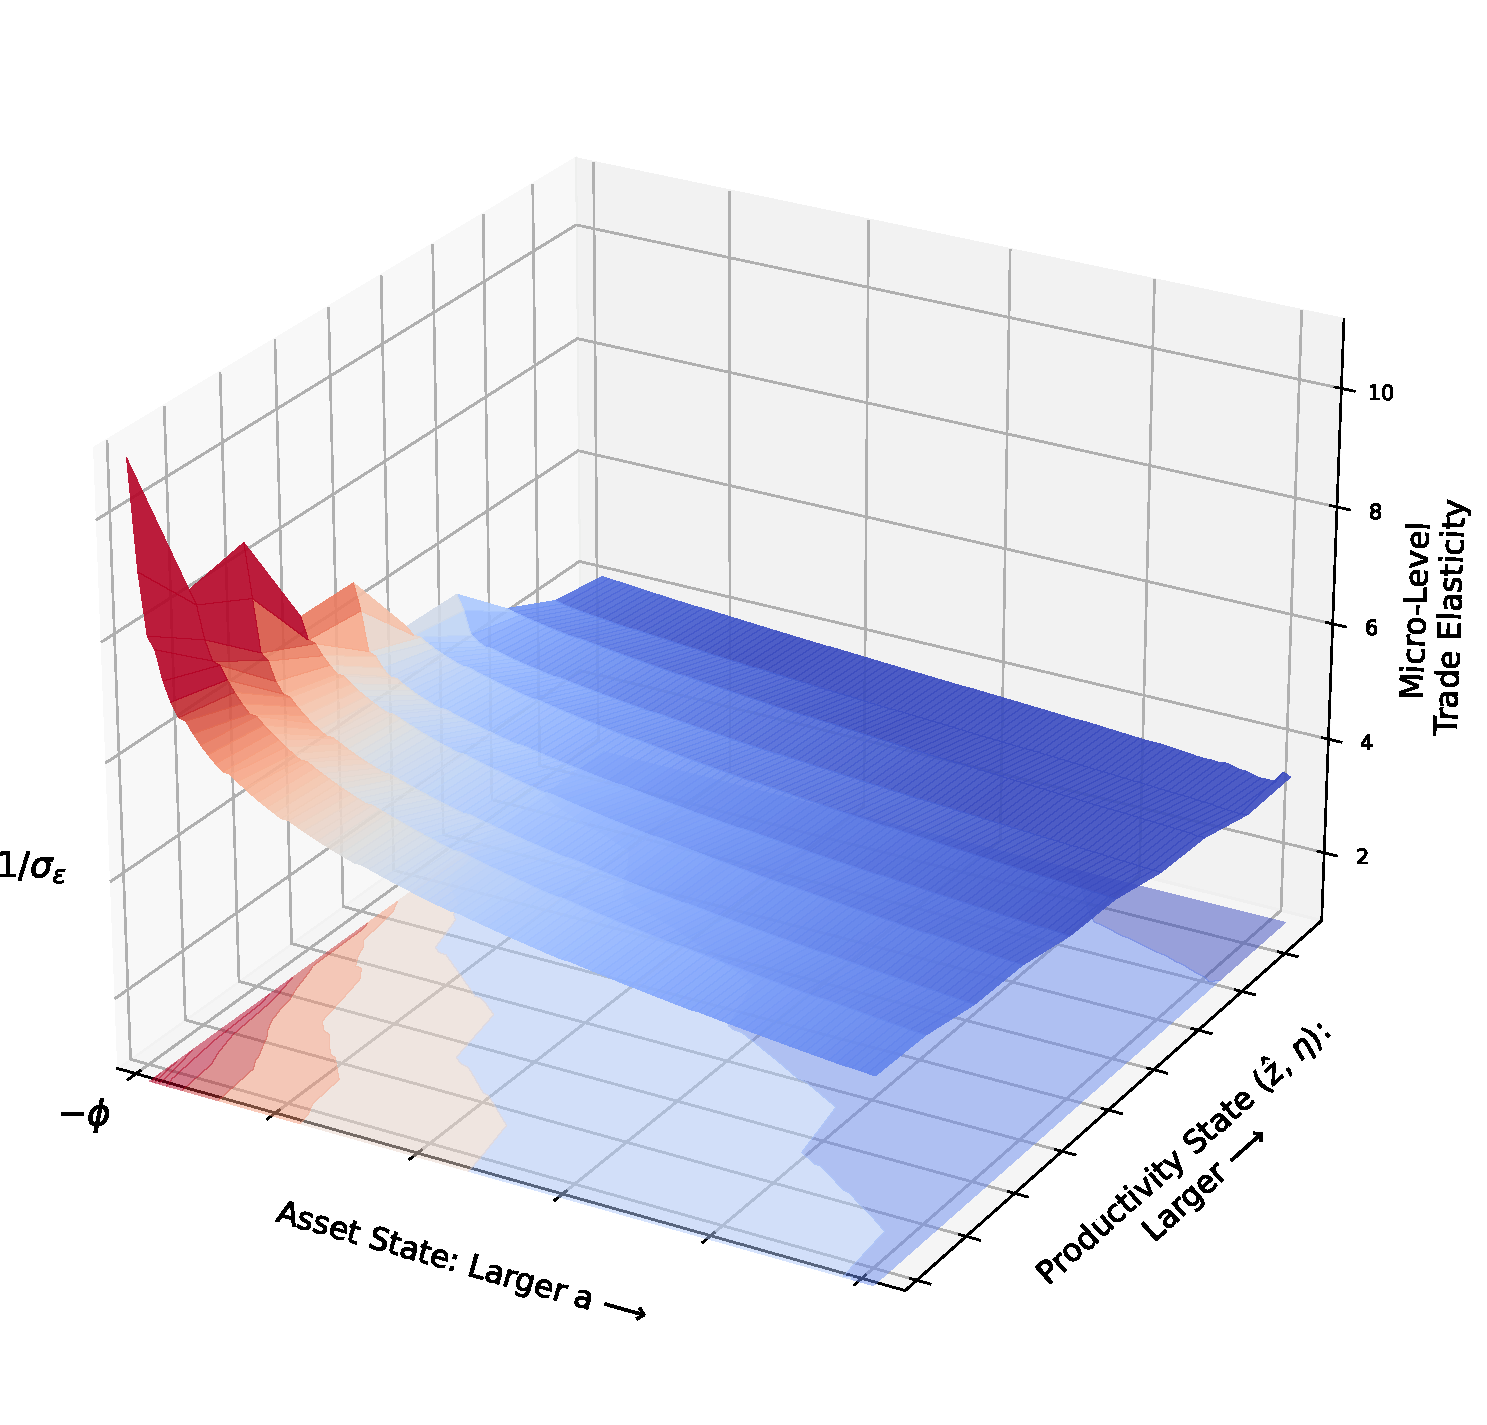
\includegraphics[scale = 0.5]{../notes/figures/micro-elasticity.pdf}}
\end{figure}
\end{frame}


\begin{frame}[t]{Trade Shares: $M_{i}(a,z,j) / M_{i}(a,z,i)$, by HH-Level State}
\vspace{-.5cm}
\begin{figure}[t]
\centerline{
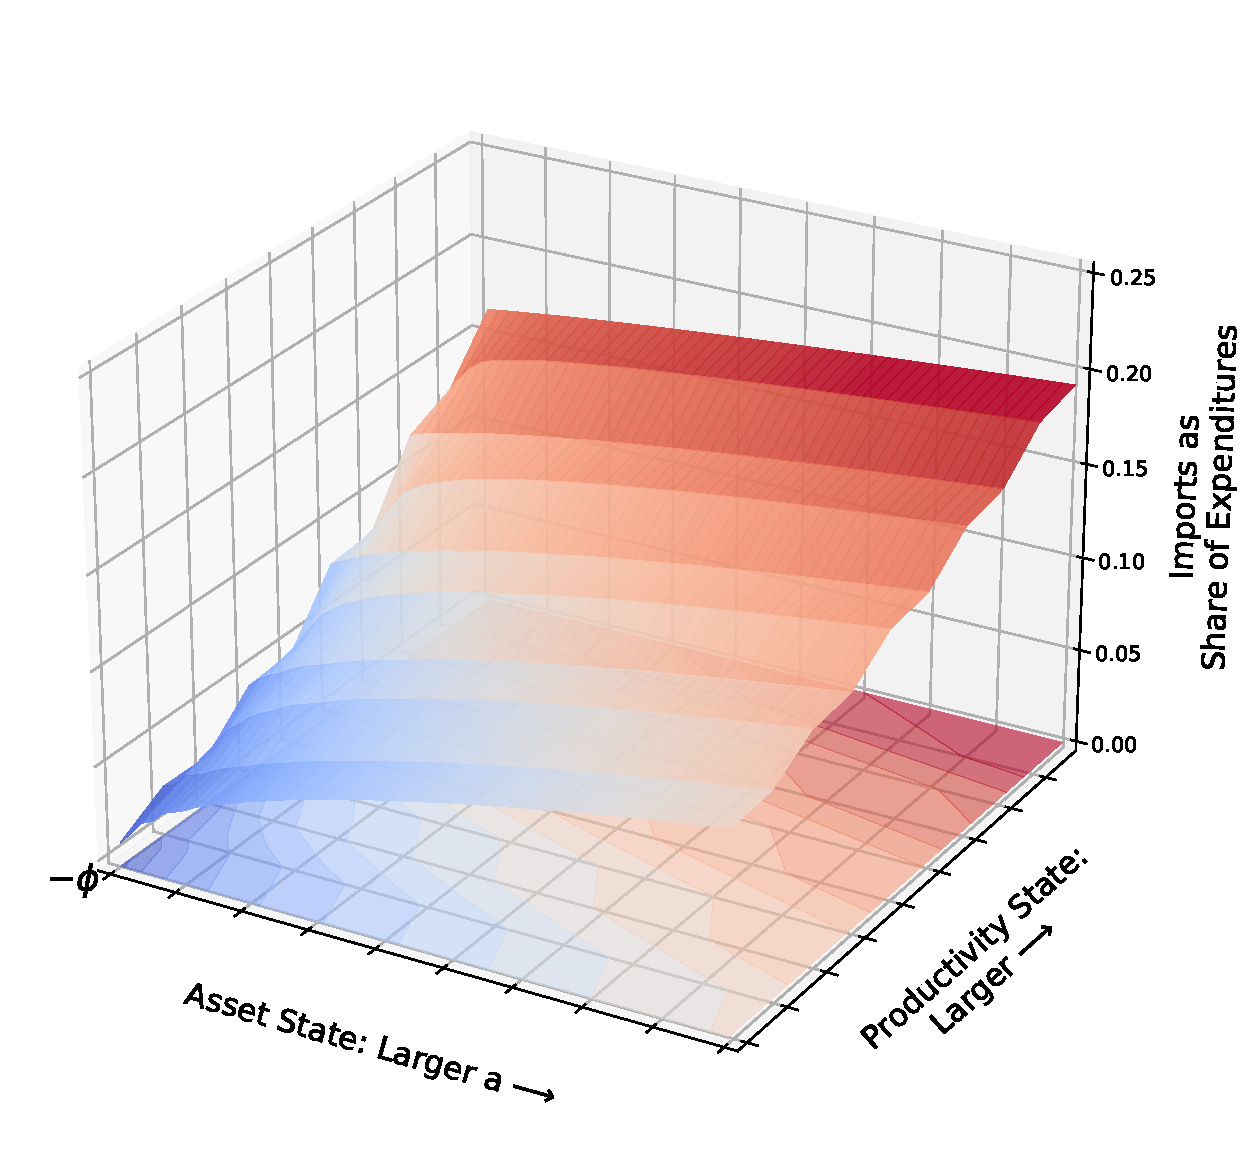
\includegraphics[scale = 0.5]{../notes/figures/trade-share.pdf}}
\end{figure}
\end{frame}


\begin{frame}[t]{HA Gains from Trade \only<1>{I}\only<2>{II}\only<3-4>{\ldots the algebra trick}\only<5>{III}}
\smallskip
\textbf{Proposition \#2: HA Welfare Gains from Trade.} The gains from trade are
\begin{align*}
\frac{\mathrm{d} W_{i}}{\mathrm{d} d_{ij} / d_{ij}} \approx \int_{z} \int_{a}  \bigg \{ \underbrace{\frac{\mathrm{d} v_i(a, z)}{\mathrm{d} d_{ij} / d_{ij}}}_{\small \mbox{gains to hh}}  + \underbrace{v_{i}(a,z) \frac{\mathrm{d} \lambda_{i}(a,z)/ \lambda_{i}(a,z)}{\mathrm{d} d_{ij} / d_{ij}}}_{\small \mbox{gains to reallocation}}   \bigg \} L_i \lambda_{i}(a,z),
\nonumber
\end{align*}
where $v_i$ is value function before realization of taste shocks; $\approx$ is about abstracting from transition. \\
\bigskip
Household-level gains are
\only<1>{
\begin{align*}
\frac{\mathrm{d} v_i(a, z)}{\mathrm{d} d_{ij} / d_{ij}} \approx \sigma_{\epsilon} \frac{\mathrm{d} \Phi_{i}(a,z) / \Phi_{i}(a,z)}{\mathrm{d} d_{ij} / d_{ij}}
\end{align*}\\
\bigskip
\medskip
Like standard trade models! It's all about how this price-index-like thing changes.
}
\only<2>{
\begin{align*}
\frac{\mathrm{d} v_i(a, z)}{\mathrm{d} d_{ij} / d_{ij}} \approx \sum_{j} \pi_{ij}(a, z) \frac{\mathrm{d} v_{i}(a,z,j)}{\mathrm{d} d_{ij}/d_{ij}}
\end{align*}\\
\bigskip
\medskip
The change in the $\Phi_{i}(a,z)$ thing (previous slide if you fell asleep) is share-weighted average of choice-specific value functions.\\
\medskip
Next step\ldots one algebra trick.
}
\only<3>{
\begin{align*}
\frac{\mathrm{d} v_i(a, z)}{\mathrm{d} d_{ij} / d_{ij}} \approx \underbrace{\sum_{j} \pi_{ij}(a, z) \bigg \{ \frac{\mathrm{d} v_{i}(a,z,j)}{\mathrm{d} d_{ij}/d_{ij}} - \frac{\mathrm{d} v_{i}(a,z,i)}{\mathrm{d} d_{ij}/d_{ij}} \bigg \}}_{\ \ \mbox{\small how relative valuations change\phantom{foo}}} \ + \  \frac{\mathrm{d}v_{i}(a,z,i)}{\mathrm{d} d_{ij}/d_{ij}}
\end{align*}
}
\only<4>{
\begin{align*}
\frac{\mathrm{d} v_i(a, z)}{\mathrm{d} d_{ij} / d_{ij}} \approx \underbrace{\sum_{j} \pi_{ij}(a, z) \bigg \{ \frac{\mathrm{d} v_{i}(a,z,j)}{\mathrm{d} d_{ij}/d_{ij}} - \frac{\mathrm{d}v_{i}(a,z,i)}{\mathrm{d} d_{ij}/d_{ij}} \bigg \}}_{ = \ \mbox{\small how the home choice, $\pi_{ii}$, changes} } \ + \  \frac{\mathrm{d}v_{i}(a,z,i)}{\mathrm{d} d_{ij}/d_{ij}}
\end{align*}\\
\bigskip
\medskip
Now recursively iterate forward in time given how $v_{ii}$ connects with $v_i$ next period.
}
\only<5>{
\begin{align*}
\frac{\mathrm{d} v_i(a, z)}{\mathrm{d} d_{ij} / d_{ij}} \approx \mathbb{E}_{z} \sum_{t = 0}^{\infty} \beta^{t} \bigg \{ -\sigma_{\epsilon} \frac{\mathrm{d} \pi_{ii}(a_{t},z_{t}) / \pi_{ii}(a_{t},z_{t})}{\mathrm{d}d_{ij} / d_{ij}} + u'(c_{i}(a_{t},z_{t},i))\bigg[ \ a_{t} \ \frac{\mathrm{d} R_{i} / p_{ii}}{\mathrm{d} d_{ij} / d_{ij}} \ \bigg] \bigg \}.
\end{align*}\\
\bigskip
\medskip
HH-level gains pick up two effects:
\begin{itemize}
\item A state contingent, ACR-like term summarizing how relative valuations across choices change.
\smallskip
\item How hh's real wealth ($+$ or $-$) change through GE effects on prices | all evaluated at the hh's marginal utility of home consumption.
\end{itemize}
}
\end{frame}

%%%%%%%%%%%%%%%%%%%%%%%%%%%%%%%%%%%%%%%%%%%%%%%%%%%%%%%%%%%%%%%%%%%%%%%%%%%%%%%%%%%%%%%%%%%%%%%%
%%%%%%%%%%%%%%%%%%%%%%%%%%%%%%%%%%%%%%%%%%%%%%%%%%%%%%%%%%%%%%%%%%%%%%%%%%%%%%%%%%%%%%%%%%%%%%%%

\begin{frame}[t]{HA Gains from Trade: $\log$ Preferences $\Rightarrow$ Separation of Trade and Heterogeneity}
\smallskip
\uncover<1->{
\textbf{Proposition \#3: Separation of Trade and Micro-Heterogeneity.} When preferences are logarithmic over the physical commodity, choice probabilities are independent of household heterogeneity
\begin{align*}
\pi_{ij}(a, z) = & \exp \left( \frac{  -\log p_{ij} }{\sigma_{\epsilon}} \right) \Bigg / \sum_{j'} \exp \left( \frac{ -\log p_{ij'} }{\sigma_{\epsilon}} \right) \ \propto \ M_{ij},
\end{align*}
and the trade elasticity is
\begin{align}
\theta = -\frac{1}{\sigma_{\epsilon}}. \nonumber
\end{align}}
\uncover<2->{And hh-level gains from trade
\begin{align*}
\frac{\mathrm{d} v_i(a, z)}{\mathrm{d} d_{ij} / d_{ij}} \approx \underbrace{-\frac{1}{\theta (1-\beta)} \times \frac{\mathrm{d} \pi_{ii} / \pi_{ii}}{\mathrm{d}d_{ij} / d_{ij}}}_{\mbox{\small ACR}} \ \ + \  \ \underbrace{\mathbb{E}_{z} \sum_{t = 0}^{\infty} \beta^{t} \bigg[ u'(c_{i}(a_{t},z_{t},i)) \ a_{t} \ \frac{\mathrm{d} R_{i} / p_{ii}}{\mathrm{d} d_{ij} / d_{ij}} \bigg ]}_{\mbox{\small exposure to finacial market}}.
\end{align*}\\}
\medskip
\only<1>{This mimics the results of \citet*{anderson1987ces}. This was not obvious to me given the environment \ldots risk, market incompleteness, borrowing constraints, etc.}
\only<2>{And we are back to \citet{arkolakis2012new} $+$ what's going on with the financial market.}
\end{frame}

%%%%%%%%%%%%%%%%%%%%%%%%%%%%%%%%%%%%%%%%%%%%%%%%%%%%%%%%%%%%%%%%%%%%%%%%%%%%%%%%%%%%%%%%%%%%%%%%
%%%%%%%%%%%%%%%%%%%%%%%%%%%%%%%%%%%%%%%%%%%%%%%%%%%%%%%%%%%%%%%%%%%%%%%%%%%%%%%%%%%%%%%%%%%%%%%%

\begin{frame}[t]{HA Trade under Efficiency}
\smallskip
\textbf{Proposition \#4: The Centralized (Efficient) Allocation.} The allocation satisfying the Centralized Planning Problem (with a utilitarian SWF and country-specific Pareto weights $\psi_i$) is:\\
\bigskip
\textbf{1.} An allocation of consumption satisfying:
\begin{align}
\psi_{i} u'(c_{i}(z,j,t) ) = \chi_{j}(t) d_{ij} \nonumber
\end{align}
where $\chi_{j}(t)$ is the multiplier on $j$ resource constraint for variety $j$,\\
\bigskip
\medskip
\textbf{2.} And variety choice probabilities:
\begin{align}
\displaystyle \pi_{ij}(t) =\exp \left( \frac{u(c_{i}(j,t)) - u'(c_{i}(j,t))c_{i}(j,t)}{\sigma_{\epsilon}}\right) \bigg / \sum_{j'}\exp \left( \frac{u(c_{i}(j',t)) - u'(c_{i}(j',t))c_{i}(j',t)}{\sigma_{\epsilon}} \right). \nonumber
\end{align}\\
\bigskip
\medskip
\textbf{1.} is a \citet{backus1993}-like condition. \\
\smallskip
\textbf{2.} is new | trade should reflect the net social benefit of buying that commodity.
\end{frame}
%%%%%%%%%%%%%%%%%%%%%%%%%%%%%%%%%%%%%%%%%%%%%%%%%%%%%%%%%%%%%%%%%%%%%%%%%%%%%%%%%%%%%%%%%%%%%%%%
%%%%%%%%%%%%%%%%%%%%%%%%%%%%%%%%%%%%%%%%%%%%%%%%%%%%%%%%%%%%%%%%%%%%%%%%%%%%%%%%%%%%%%%%%%%%%%%%

\begin{frame}[t]{HA Gains from Trade under Efficiency}
\smallskip
\textbf{Proposition \#5: Trade Elasticities and Welfare Gains in the Efficient Allocation} The trade elasticity between $i,j$ in the efficient allocation is:
\begin{align}
\theta_{ij} =  -\frac{1}{\sigma_{\epsilon}} \bigg [ u'(c_{ij}) c_{ij} \bigg]. \nonumber
\end{align}\\
\bigskip
And the welfare gains from a reduction in trade costs between $i,j$ are
\begin{align}
\frac{\mathrm{d} W}{\mathrm{d} d_{ij} / d_{ij}} = \frac{\partial W}{\partial d_{ij} / d_{ij}} = \frac{\psi_{i}}{1-\beta} \times u'(c_{ij}) c_{ij} \pi_{ij} L_i, \nonumber
\end{align}
which is the discounted, weighted, direct effect from relaxing the resource constraint.\\
\bigskip
Two comments:
\begin{itemize}
\smallskip
\item Mimics the results of \citet{AtkesonBurstein2010} but with household (not firm) heterogeneity.
\smallskip
\item With $\log$ preferences the direct effect is equivalent to \citet{arkolakis2012new}.
\end{itemize}
\end{frame}

%%%%%%%%%%%%%%%%%%%%%%%%%%%%%%%%%%%%%%%%%%%%%%%%%%%%%%%%%%%%%%%%%%%%%%%%%%%%%%%%%%%%%%%%%%%%%%%%
%%%%%%%%%%%%%%%%%%%%%%%%%%%%%%%%%%%%%%%%%%%%%%%%%%%%%%%%%%%%%%%%%%%%%%%%%%%%%%%%%%%%%%%%%%%%%%%%

\begin{frame}[t]{Quantitative Analysis}
\smallskip
\smallskip
This is what I'll do today\ldots\\
\bigskip
\textbf{1.} Calibrate my model using my ``gravity as a guide'' approach on the 19 country data set of \citet{eaton2002technology}. \\
\bigskip
\textbf{2.} Some gains from trade type calculations.\\
\bigskip
\textbf{3.} Trade in the efficient allocation vs. the decentralized allocation.\\
\end{frame}

%%%%%%%%%%%%%%%%%%%%%%%%%%%%%%%%%%%%%%%%%%%%%%%%%%%%%%%%%%%%%%%%%%%%%%%%%%%%%%%%%%%%%%%%%%%%%%%%
%%%%%%%%%%%%%%%%%%%%%%%%%%%%%%%%%%%%%%%%%%%%%%%%%%%%%%%%%%%%%%%%%%%%%%%%%%%%%%%%%%%%%%%%%%%%%%%%

\begin{frame}[t]{Household Parameters}
\smallskip
Parameters common across countries:
\begin{itemize}
\smallskip
\item CRRA for $u$ with relative risk aversion $\gamma = 1.5$.\\
\smallskip
\item Earnings process is a mixture of a persistent and transitory component and calibrated as in\\ \citet*{krueger2016macroeconomics}.
\smallskip
\item Discount factor $\beta$ jiggled to target a world interest rate of $1.5 \%$ in financial globalization case.
\end{itemize}
\bigskip
Parameters scaled across countries to deliver balanced-growth-like properties.
\begin{itemize}
\smallskip
\item Set $\sigma_{\epsilon,i} = \sigma_{\epsilon}\times A_i^{1-\gamma}$ and $\sigma_{\epsilon} = 0.25$.\\ In a $\log$ model corresponds with a trade elasticity of 4.
\medskip
\item Set the borrowing constraint so $\phi_{i} = \phi \times A_i$ where $\phi = 0.50$.\\
 Interpretation: the constraint $=$ 50 \% of average, autarky labor income.
\end{itemize}
\end{frame}

%%%%%%%%%%%%%%%%%%%%%%%%%%%%%%%%%%%%%%%%%%%%%%%%%%%%%%%%%%%%%%%%%%%%%%%%%%%%%%%%%%%%%%%%%%%%%%%%
%%%%%%%%%%%%%%%%%%%%%%%%%%%%%%%%%%%%%%%%%%%%%%%%%%%%%%%%%%%%%%%%%%%%%%%%%%%%%%%%%%%%%%%%%%%%%%%%

\begin{frame}[t]{County Specific Parameters | Using Gravity as a Guide}
\smallskip
\only<1>{
The problem: no closed form map from trade flows to parameters as in standard trade models. But I want the model to replicate the geographic pattern of activity seen in the data.}
\only<2>{The solution: use the gravity regression ``as a guide'' where I estimate parameters of the model so that the regression coefficients run on my model's data match that seen in the data.}
\medskip
\uncover<2->{
\begin{itemize}
\smallskip
\item Step 0. Impose a trade cost function to reduce the parameter space
\begin{align}
\log d_{ij} = d_{k} + b + l + e_{h} + m_{i}. \nonumber
\end{align}
\smallskip
\item Step 1. Run this gravity regression on the data
\begin{align}
\log \left( {\frac{M_{ij}}{M_{ii}}} \right) = {Im_{i}} + {Ex_{j}} + {d_{k}} + {b} + {l} + {e_{h}} + \delta_{ij}. \nonumber
\end{align}
\smallskip
\item Step 2. Guess TFP terms and coefficients on the trade cost function, compute an equilibrium, run the same regression from above on model generated data.
\smallskip
\item Step 3. Evaluate difference between model and data and update parameters until convergence.
\end{itemize}
}
\end{frame}

%%%%%%%%%%%%%%%%%%%%%%%%%%%%%%%%%%%%%%%%%%%%%%%%%%%%%%%%%%%%%%%%%%%%%%%%%%%%%%%%%%%%%%%%%%%%%%%%
%%%%%%%%%%%%%%%%%%%%%%%%%%%%%%%%%%%%%%%%%%%%%%%%%%%%%%%%%%%%%%%%%%%%%%%%%%%%%%%%%%%%%%%%%%%%%%%%



%%%%%%%%%%%%%%%%%%%%%%%%%%%%%%%%%%%%%%%%%%%%%%%%%%%%%%%%%%%%%%%%%%%%%%%%%%%%%%%%%%%%%%%%%%%%%%%%
%%%%%%%%%%%%%%%%%%%%%%%%%%%%%%%%%%%%%%%%%%%%%%%%%%%%%%%%%%%%%%%%%%%%%%%%%%%%%%%%%%%%%%%%%%%%%%%%

\begin{frame}[t]{Bilateral Trade: Model vs. Data}
\begin{figure}[!t]
\centering{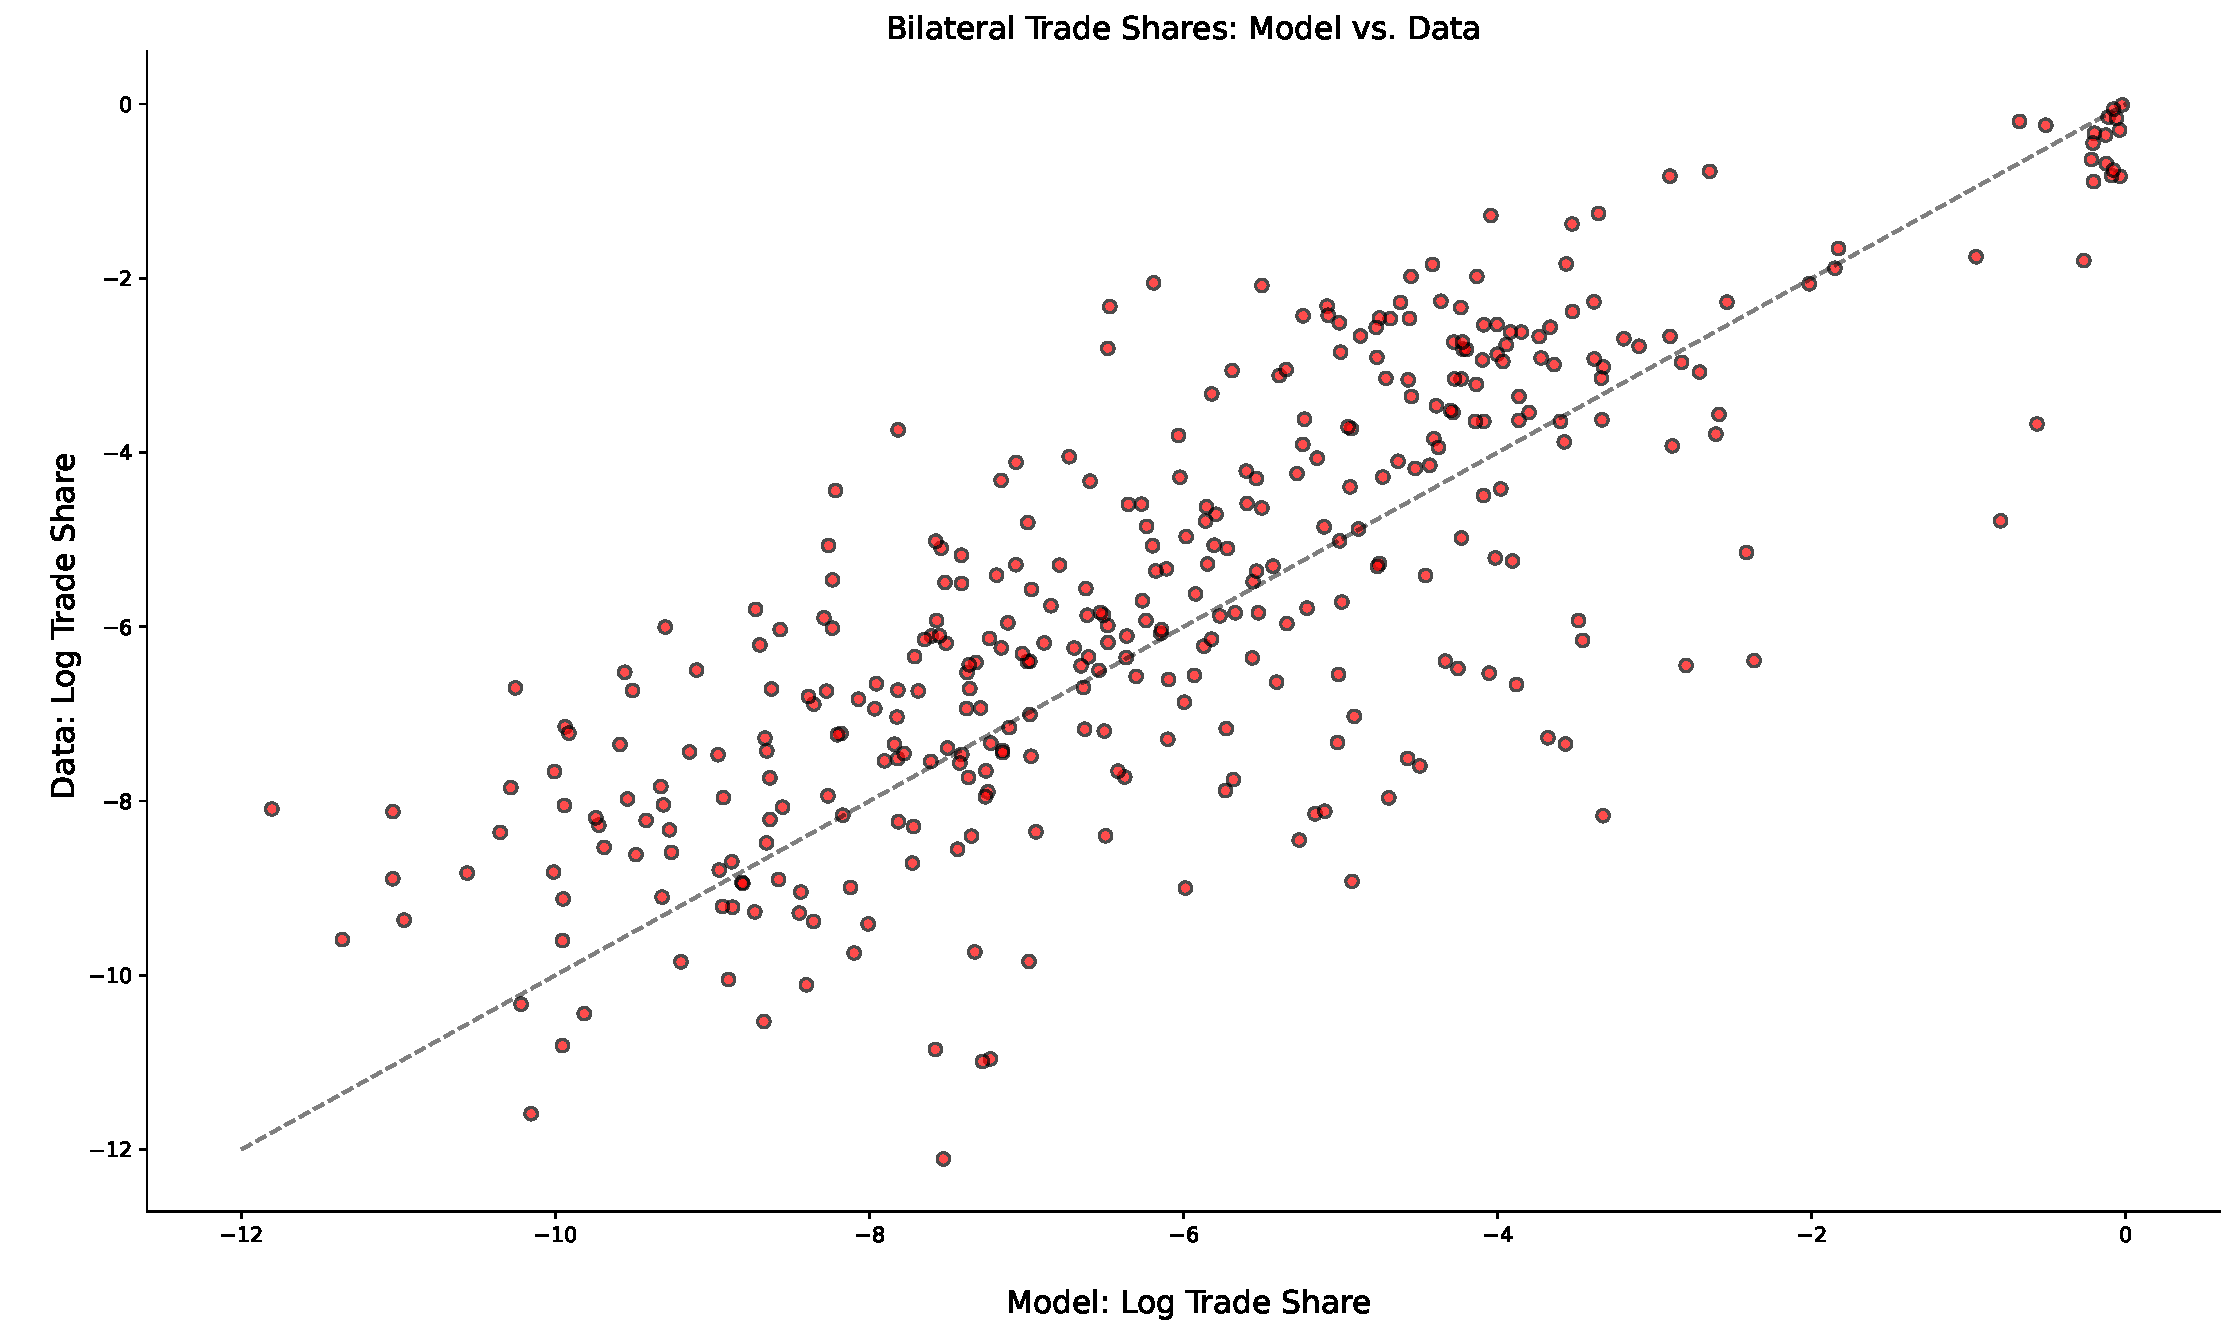
\includegraphics[scale = .35]{../notes/figures/trade-fit.pdf}}
\end{figure}
\end{frame}

%%%%%%%%%%%%%%%%%%%%%%%%%%%%%%%%%%%%%%%%%%%%%%%%%%%%%%%%%%%%%%%%%%%%%%%%%%%%%%%%%%%%%%%%%%%%%%%%
%%%%%%%%%%%%%%%%%%%%%%%%%%%%%%%%%%%%%%%%%%%%%%%%%%%%%%%%%%%%%%%%%%%%%%%%%%%%%%%%%%%%%%%%%%%%%%%%

\begin{frame}[t]
\frametitle{Estimates of Geographic Barriers}
\begin{table}[t]
\small
\begin{center}
\refstepcounter{table}
\setlength {\tabcolsep}{5.5mm}
\renewcommand{\arraystretch}{1.10}\label{tb-grav-est}
\begin{tabular}[t]{l c c c}
\multicolumn{4}{c}{{\normalsize\textbf{Table \ref{tb-grav-est}: Estimation Results}} }
\\\hline \hline
& & \multicolumn{2}{c}{\textbf{HAT-Model}}  \\
\cmidrule(lr){3-4}
Barrier& Moment & Model Fit & Parameter \\
\hline $[0,375)$                &$-3.10 $           & $-3.10 $              & $2.35$           \\
$[375,750)$                     &$-3.67 $           & $-3.67 $              & $2.81$           \\
$[750,1500)$                    &$-4.03 $           & $-4.03 $              & $3.09$           \\
$[1500,3000)$                   &$-4.22 $           & $-4.22 $              & $3.23$           \\
$[3000,6000)$                   &$-6.06 $           & $-6.06 $              & $4.88$           \\
$[6000,\mbox{maximum}]$         &$-6.56 $           & $-6.56 $              & $5.69$           \\
Shared border                   &$\phantom{-}0.30$  & $\phantom{-}0.30$     & $0.91$  \\
Language                        &$\phantom{-}0.51$  & $\phantom{-}0.51$     & $0.87$  \\
EFTA                            &$\phantom{-}0.04$  & $\phantom{-}0.04$     & $0.98$  \\
European Community              &$\phantom{-}0.54$  & $\phantom{-}0.54$     & $0.89$  \\
\hline
\end{tabular}
\\[0.5ex]
\parbox{4.2in}{\footnotesize \textbf{Note:} The first column reports data moments the HAT-model targets. The second reports the model moments. The third column reports the estimated parameter values.}
\end{center}
\end{table}
\bigskip
Far distances $\approx$ 10 percent less expensive than standard models would predict.
\end{frame}

%%%%%%%%%%%%%%%%%%%%%%%%%%%%%%%%%%%%%%%%%%%%%%%%%%%%%%%%%%%%%%%%%%%%%%%%%%%%%%%%%%%%%%%%%%%%%%%%
%%%%%%%%%%%%%%%%%%%%%%%%%%%%%%%%%%%%%%%%%%%%%%%%%%%%%%%%%%%%%%%%%%%%%%%%%%%%%%%%%%%%%%%%%%%%%%%%

\begin{frame}[t]{US Trade Elasticities: $-\theta_{us,j}$}
\begin{figure}[!t]
\centering{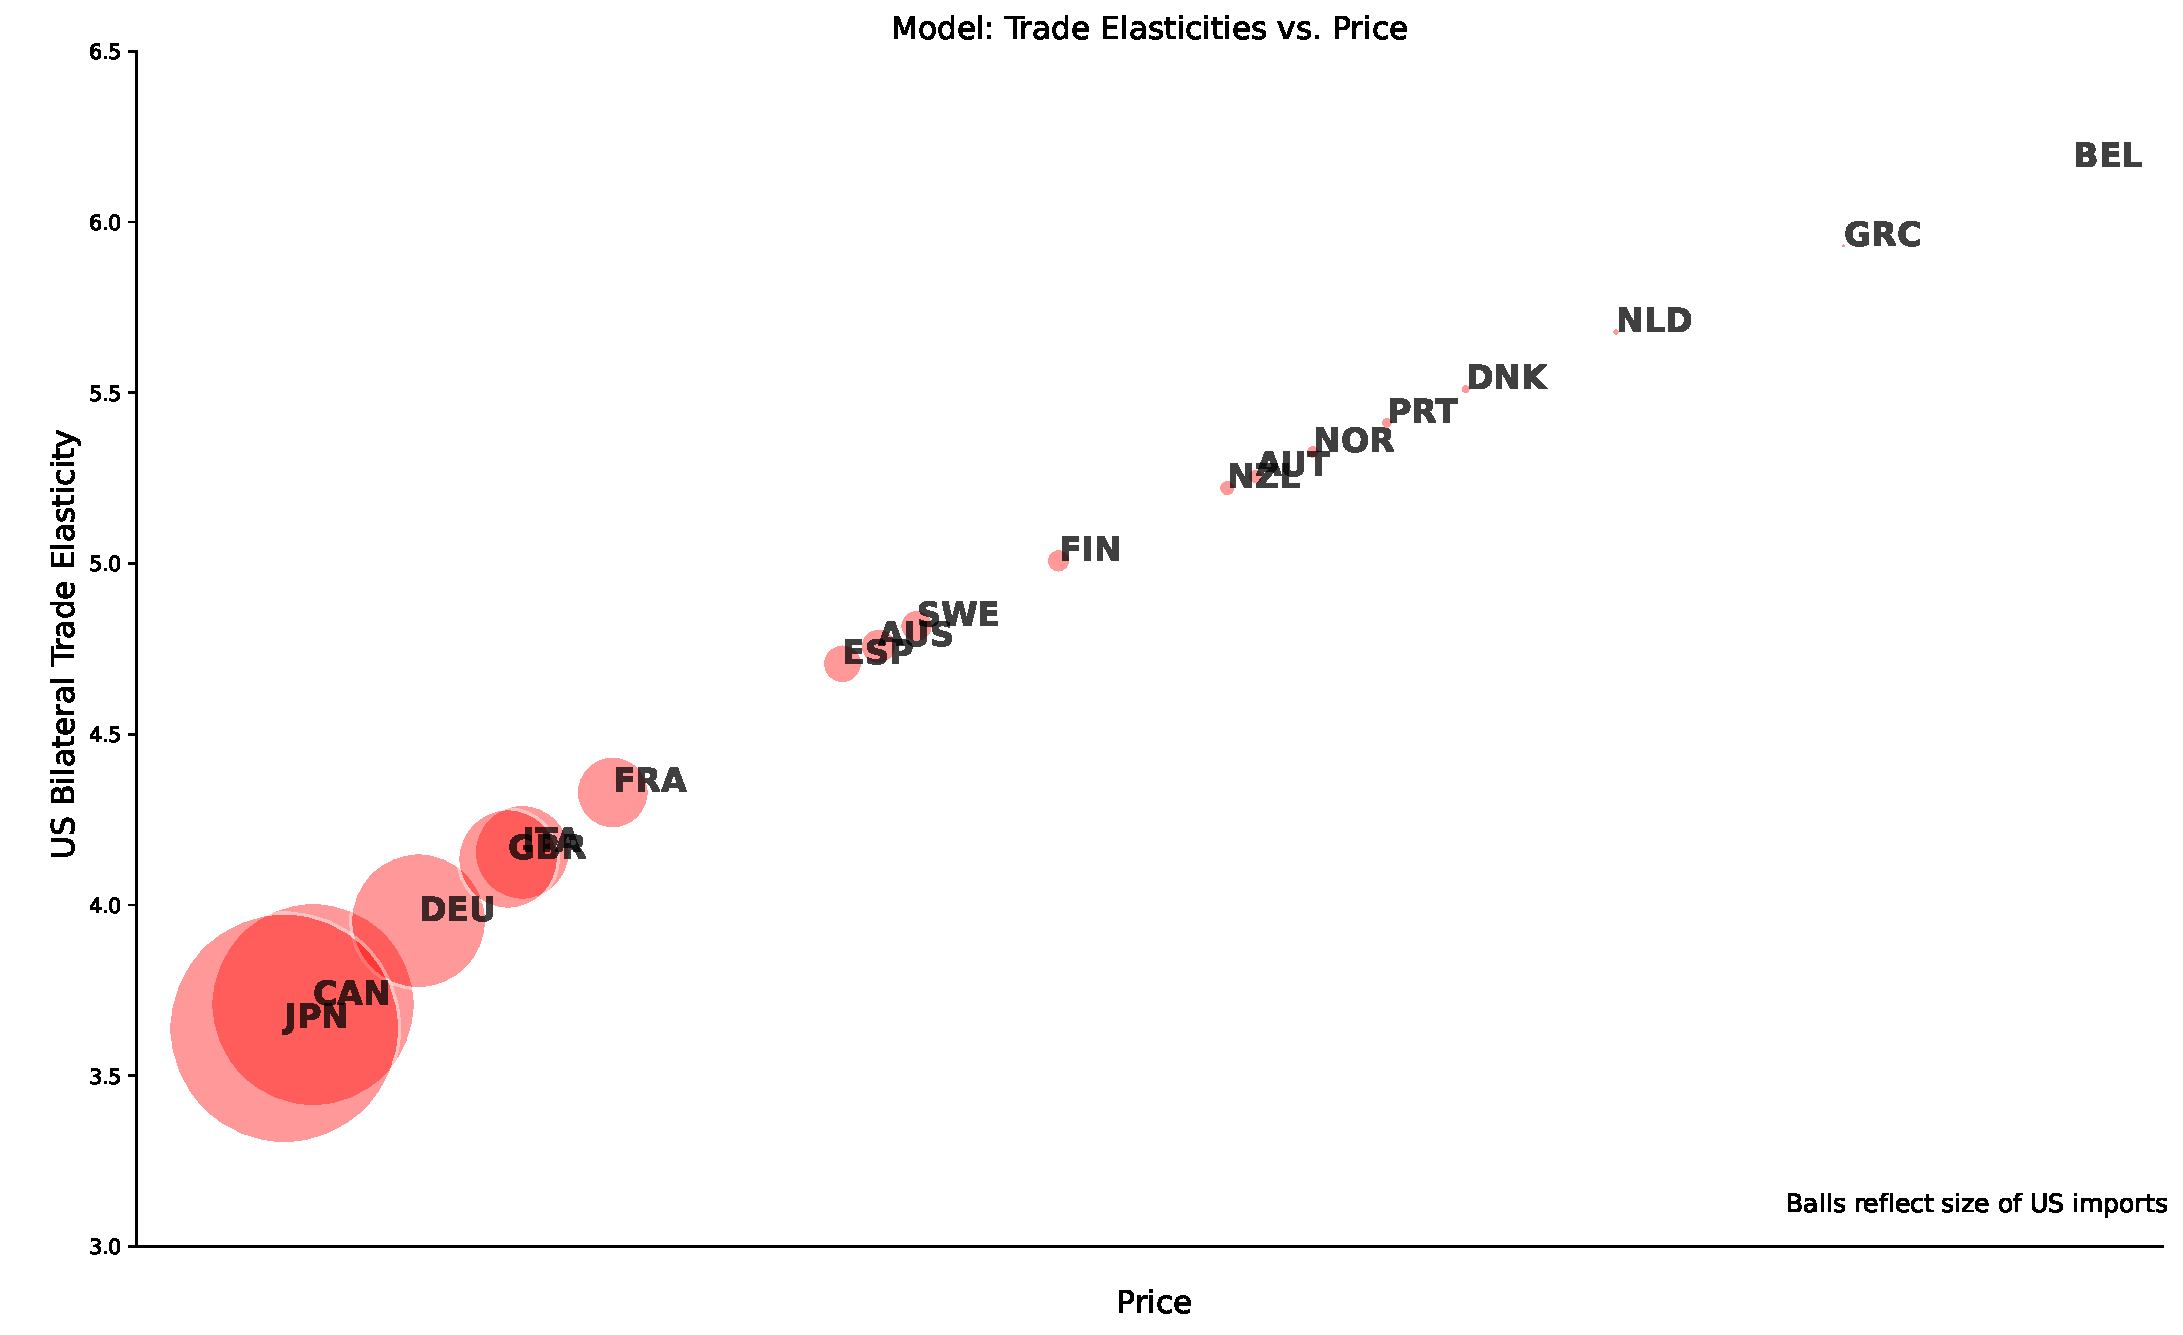
\includegraphics[scale = .35]{../notes/figures/us-elasticity.pdf}}
\end{figure}
\end{frame}
%%%%%%%%%%%%%%%%%%%%%%%%%%%%%%%%%%%%%%%%%%%%%%%%%%%%%%%%%%%%%%%%%%%%%%%%%%%%%%%%%%%%%%%%%%%%%%%%
%%%%%%%%%%%%%%%%%%%%%%%%%%%%%%%%%%%%%%%%%%%%%%%%%%%%%%%%%%%%%%%%%%%%%%%%%%%%%%%%%%%%%%%%%%%%%%%%

\begin{frame}[t]{Gains from Trade}
\smallskip
Two ideas I want to illustrate:\\
\medskip
\textbf{1.} You pick the market, you pick a person.\\
\medskip
\textbf{2.} GE effects have distributional consequences.\\
\bigskip
Next slides:\\
\smallskip
10\% reduction to US import trade cost on different source markets: Japan (big), France (medium). Focus on US welfare and break it down by\ldots
\begin{itemize}
\smallskip
\item[A.] Fix $R$ \& $w$, so what is direct effect of change in trade cost,
\smallskip
\item[B.] $R$ \& $w$ adjust to clear goods and asset markets.
\end{itemize}
\end{frame}

\begin{frame}[t]{U.S. Welfare: 10\% Reduction to Japan }
\begin{figure}[!t]
\begin{subfigure}{}
    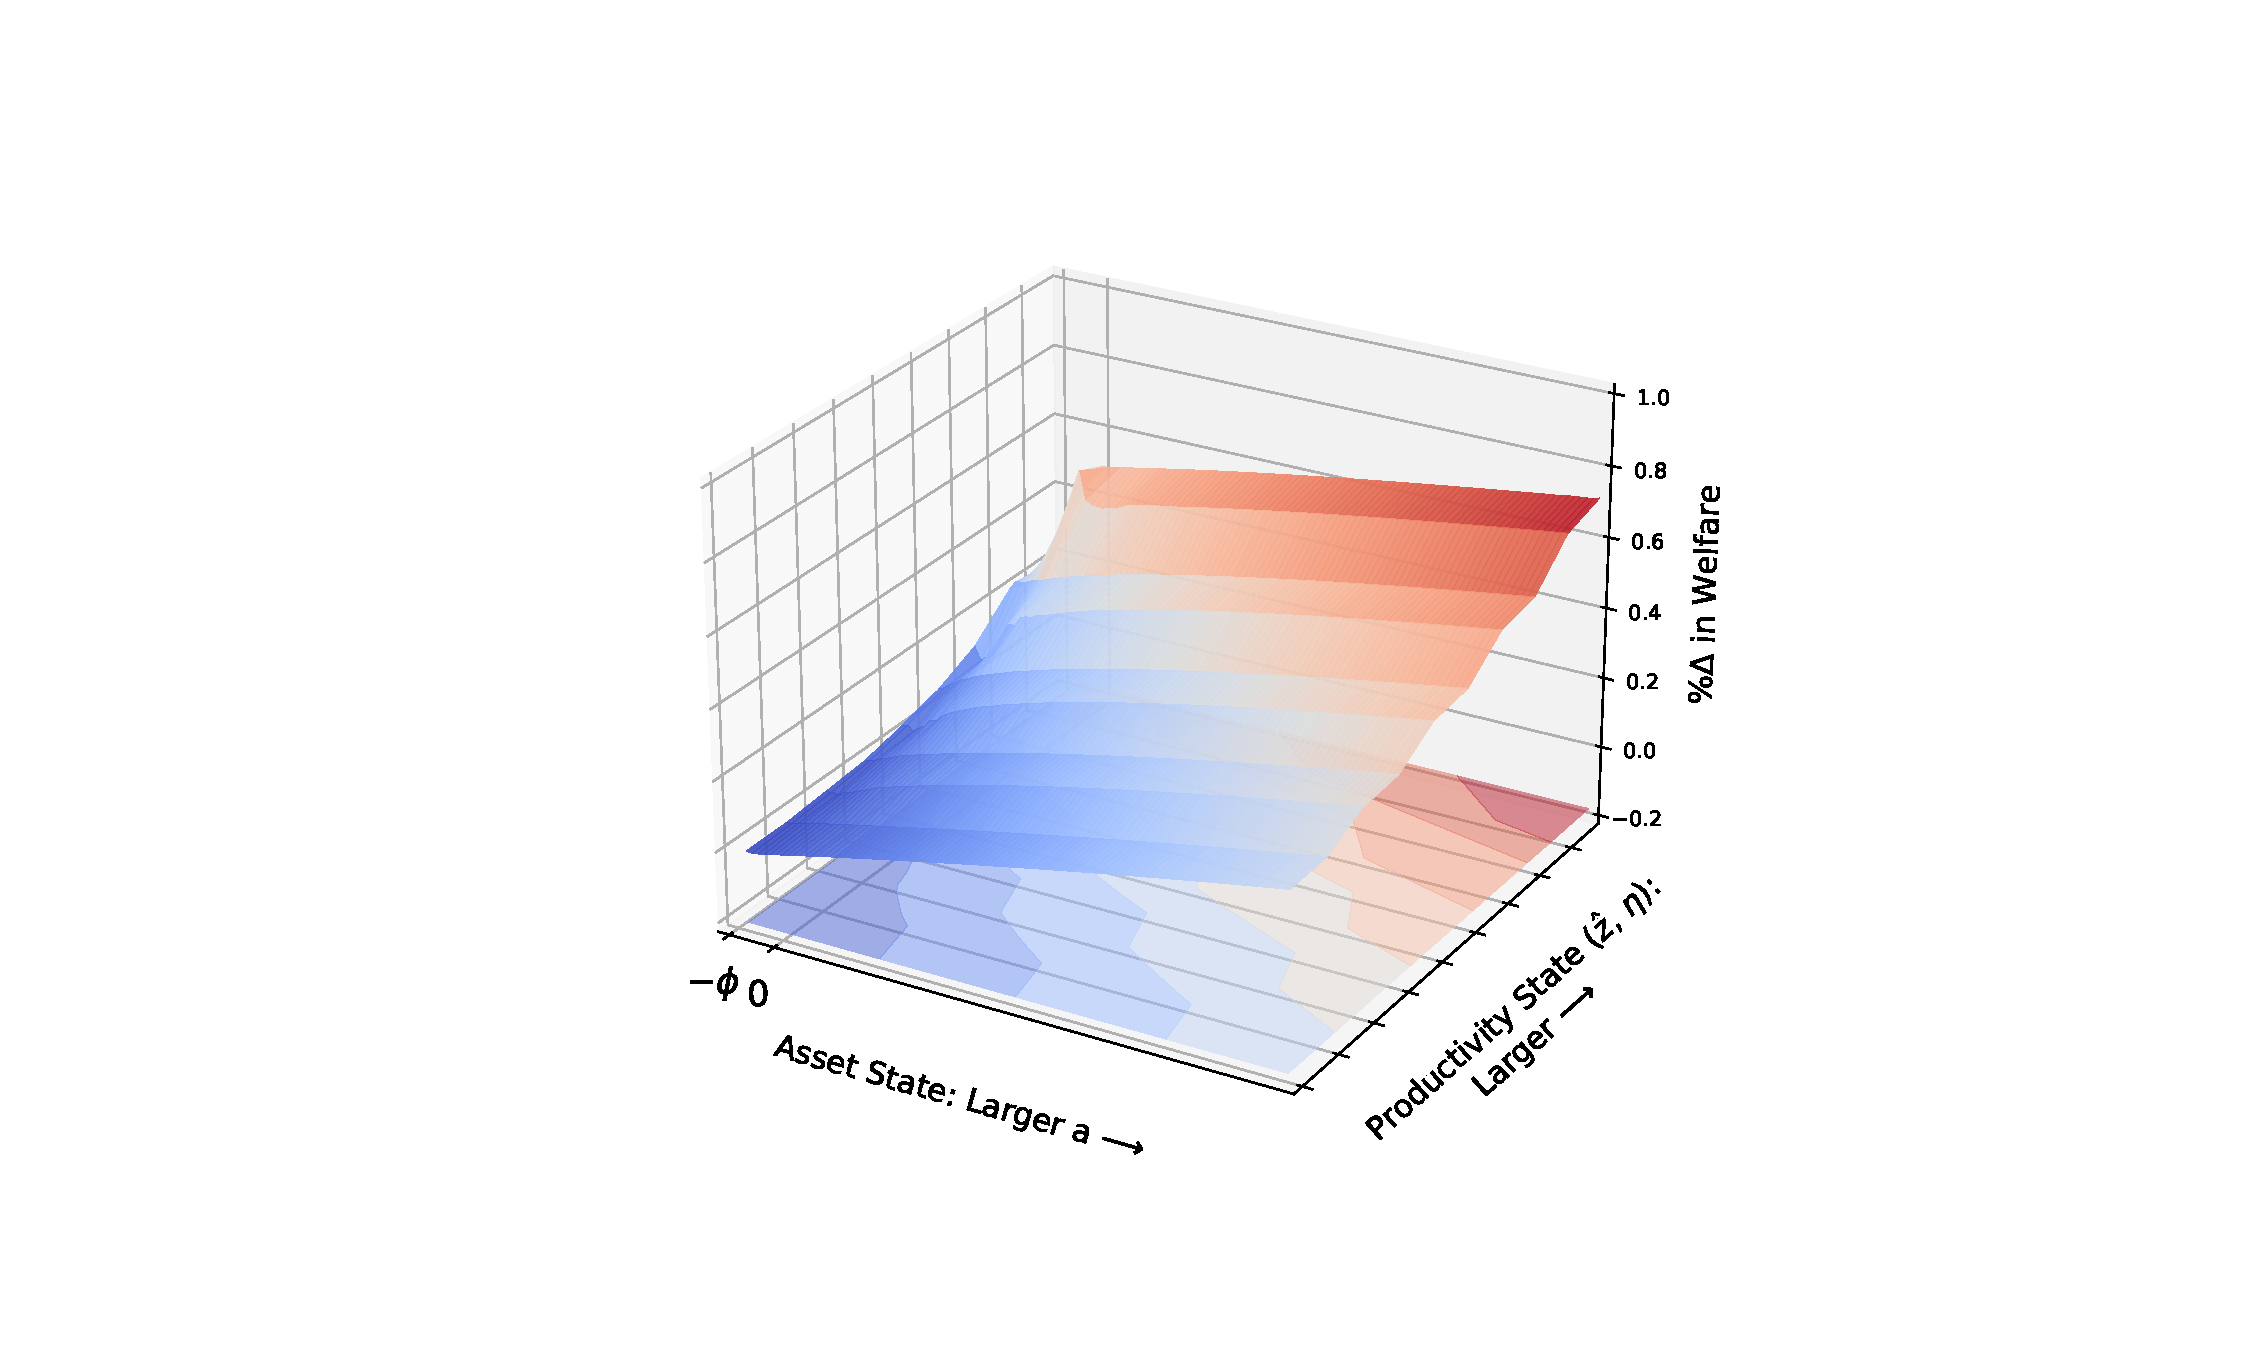
\includegraphics[scale = 0.35]{../notes/figures/welfare-jpn-fix-p.pdf}
\end{subfigure}
\begin{subfigure}{}
    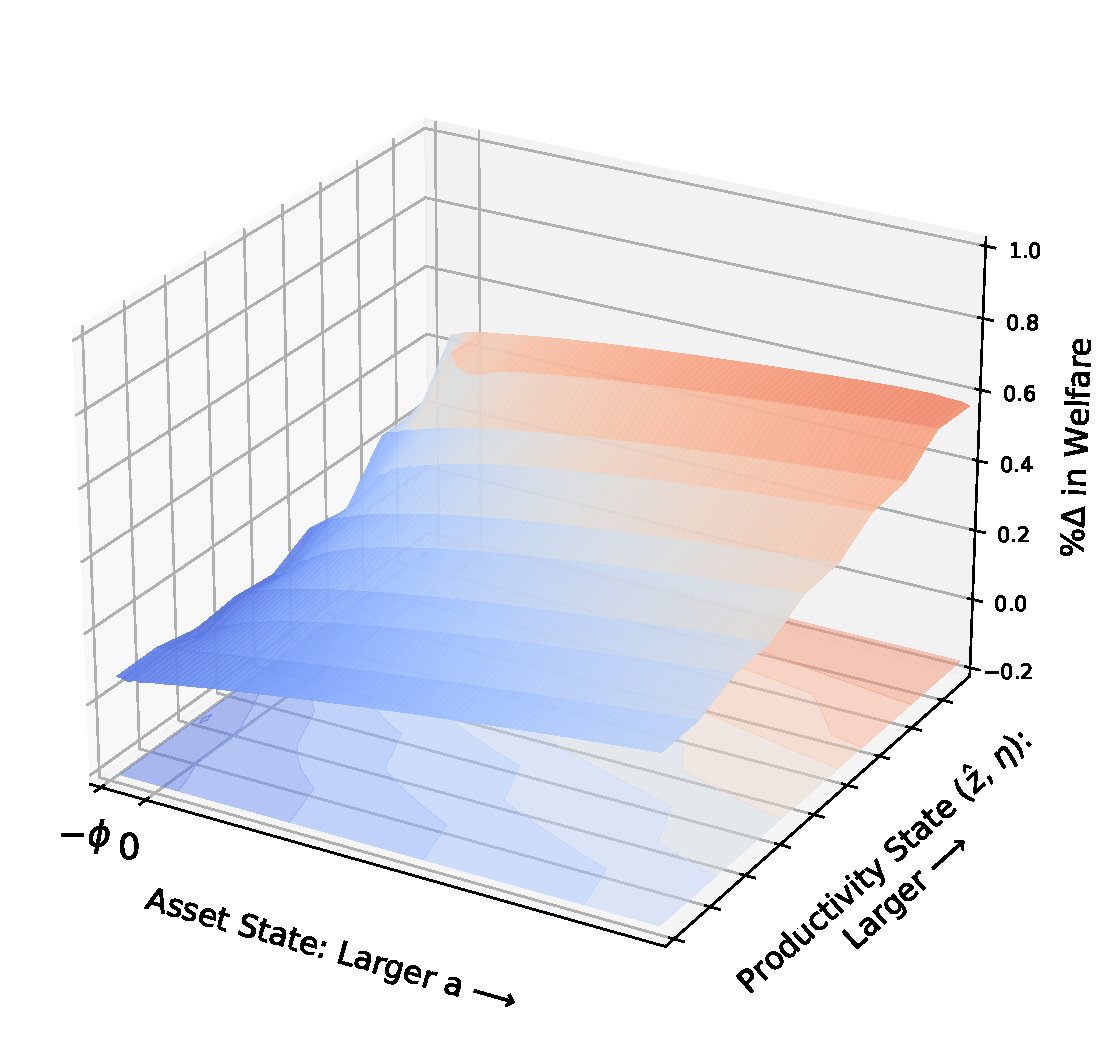
\includegraphics[scale = 0.35]{../notes/figures/welfare-jpn-ge.pdf}
\end{subfigure}
\end{figure}
\bigskip
\textbf{1.} Most gain | but trade is very pro-rich. \textbf{2.} $R$ fell $\Rightarrow$ the poor who don't benefit directly from trade with Japan gain (left vs. right panel).
\end{frame}

%%%%%%%%%%%%%%%%%%%%%%%%%%%%%%%%%%%%%%%%%%%%%%%%%%%%%%%%%%%%%%%%%%%%%%%%%%%%%%%%%%%%%%%%%%%%%%%%
%%%%%%%%%%%%%%%%%%%%%%%%%%%%%%%%%%%%%%%%%%%%%%%%%%%%%%%%%%%%%%%%%%%%%%%%%%%%%%%%%%%%%%%%%%%%%%%

\begin{frame}[t]{U.S. Welfare: 10\% Reduction to France }
\begin{figure}[!t]
\begin{subfigure}{}
    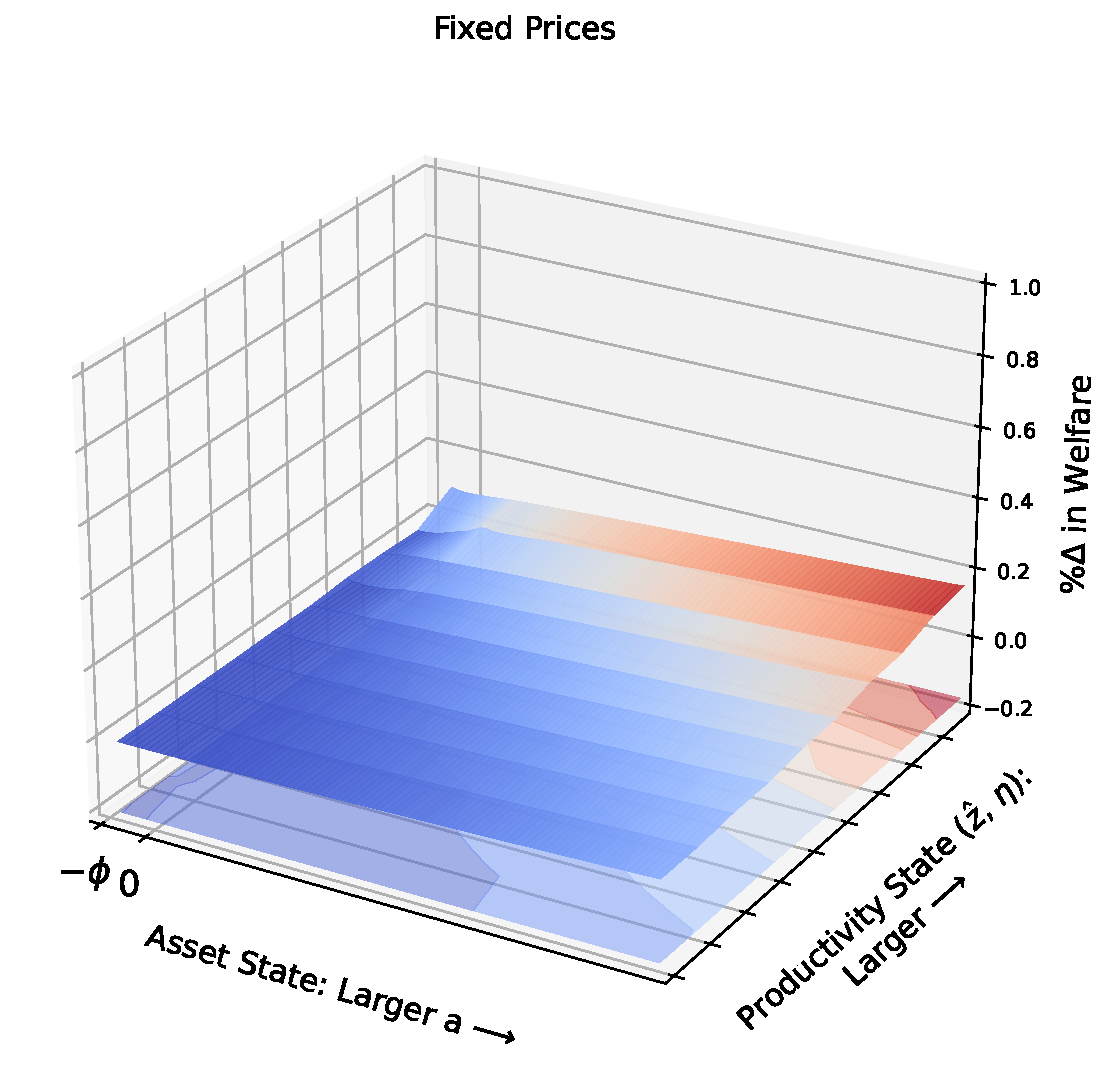
\includegraphics[scale = 0.35]{../notes/figures/welfare-france-fix-p.pdf}
\end{subfigure}
\begin{subfigure}{}
    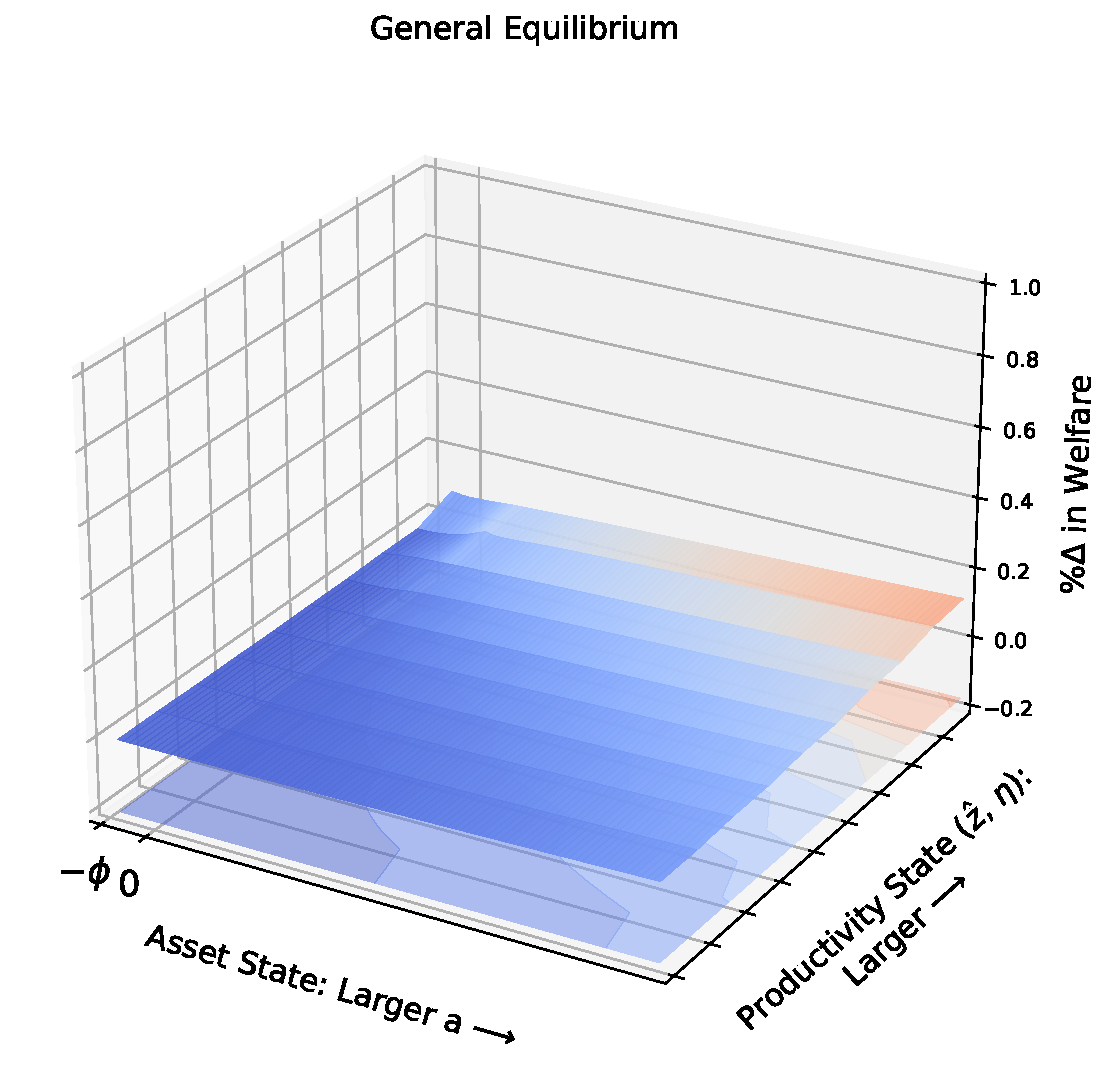
\includegraphics[scale = 0.35]{../notes/figures/welfare-france-ge.pdf}
\end{subfigure}
\end{figure}
\bigskip
Relative to Japan: Gains from trade smaller, very concentrated on the rich.
\end{frame}

%%%%%%%%%%%%%%%%%%%%%%%%%%%%%%%%%%%%%%%%%%%%%%%%%%%%%%%%%%%%%%%%%%%%%%%%%%%%%%%%%%%%%%%%%%%%%%%%
%%%%%%%%%%%%%%%%%%%%%%%%%%%%%%%%%%%%%%%%%%%%%%%%%%%%%%%%%%%%%%%%%%%%%%%%%%%%%%%%%%%%%%%%%%%%%%%%
\begin{frame}[t]{Efficient Trade}
\smallskip
The previous slides suggest that being exposed / liberalizing with some markets is better than others.\\
\medskip
What is the first-best pattern of trade?\\
\bigskip
How I answer this question:
\begin{itemize}
\smallskip
\item Take a stand on country-specific Pareto weights | I set them proportional to a country's TFP.\\
    Why? P2C2E in a slide.
\smallskip
\item Then given calibrated parameter values, compute the efficient allocation in Proposition \#4.
\end{itemize}
\end{frame}

%%%%%%%%%%%%%%%%%%%%%%%%%%%%%%%%%%%%%%%%%%%%%%%%%%%%%%%%%%%%%%%%%%%%%%%%%%%%%%%%%%%%%%%%%%%%%%%%
%%%%%%%%%%%%%%%%%%%%%%%%%%%%%%%%%%%%%%%%%%%%%%%%%%%%%%%%%%%%%%%%%%%%%%%%%%%%%%%%%%%%%%%%%%%%%%%%

\begin{frame}[t]{Efficient Trade}

\begin{figure}[!t]
\centering{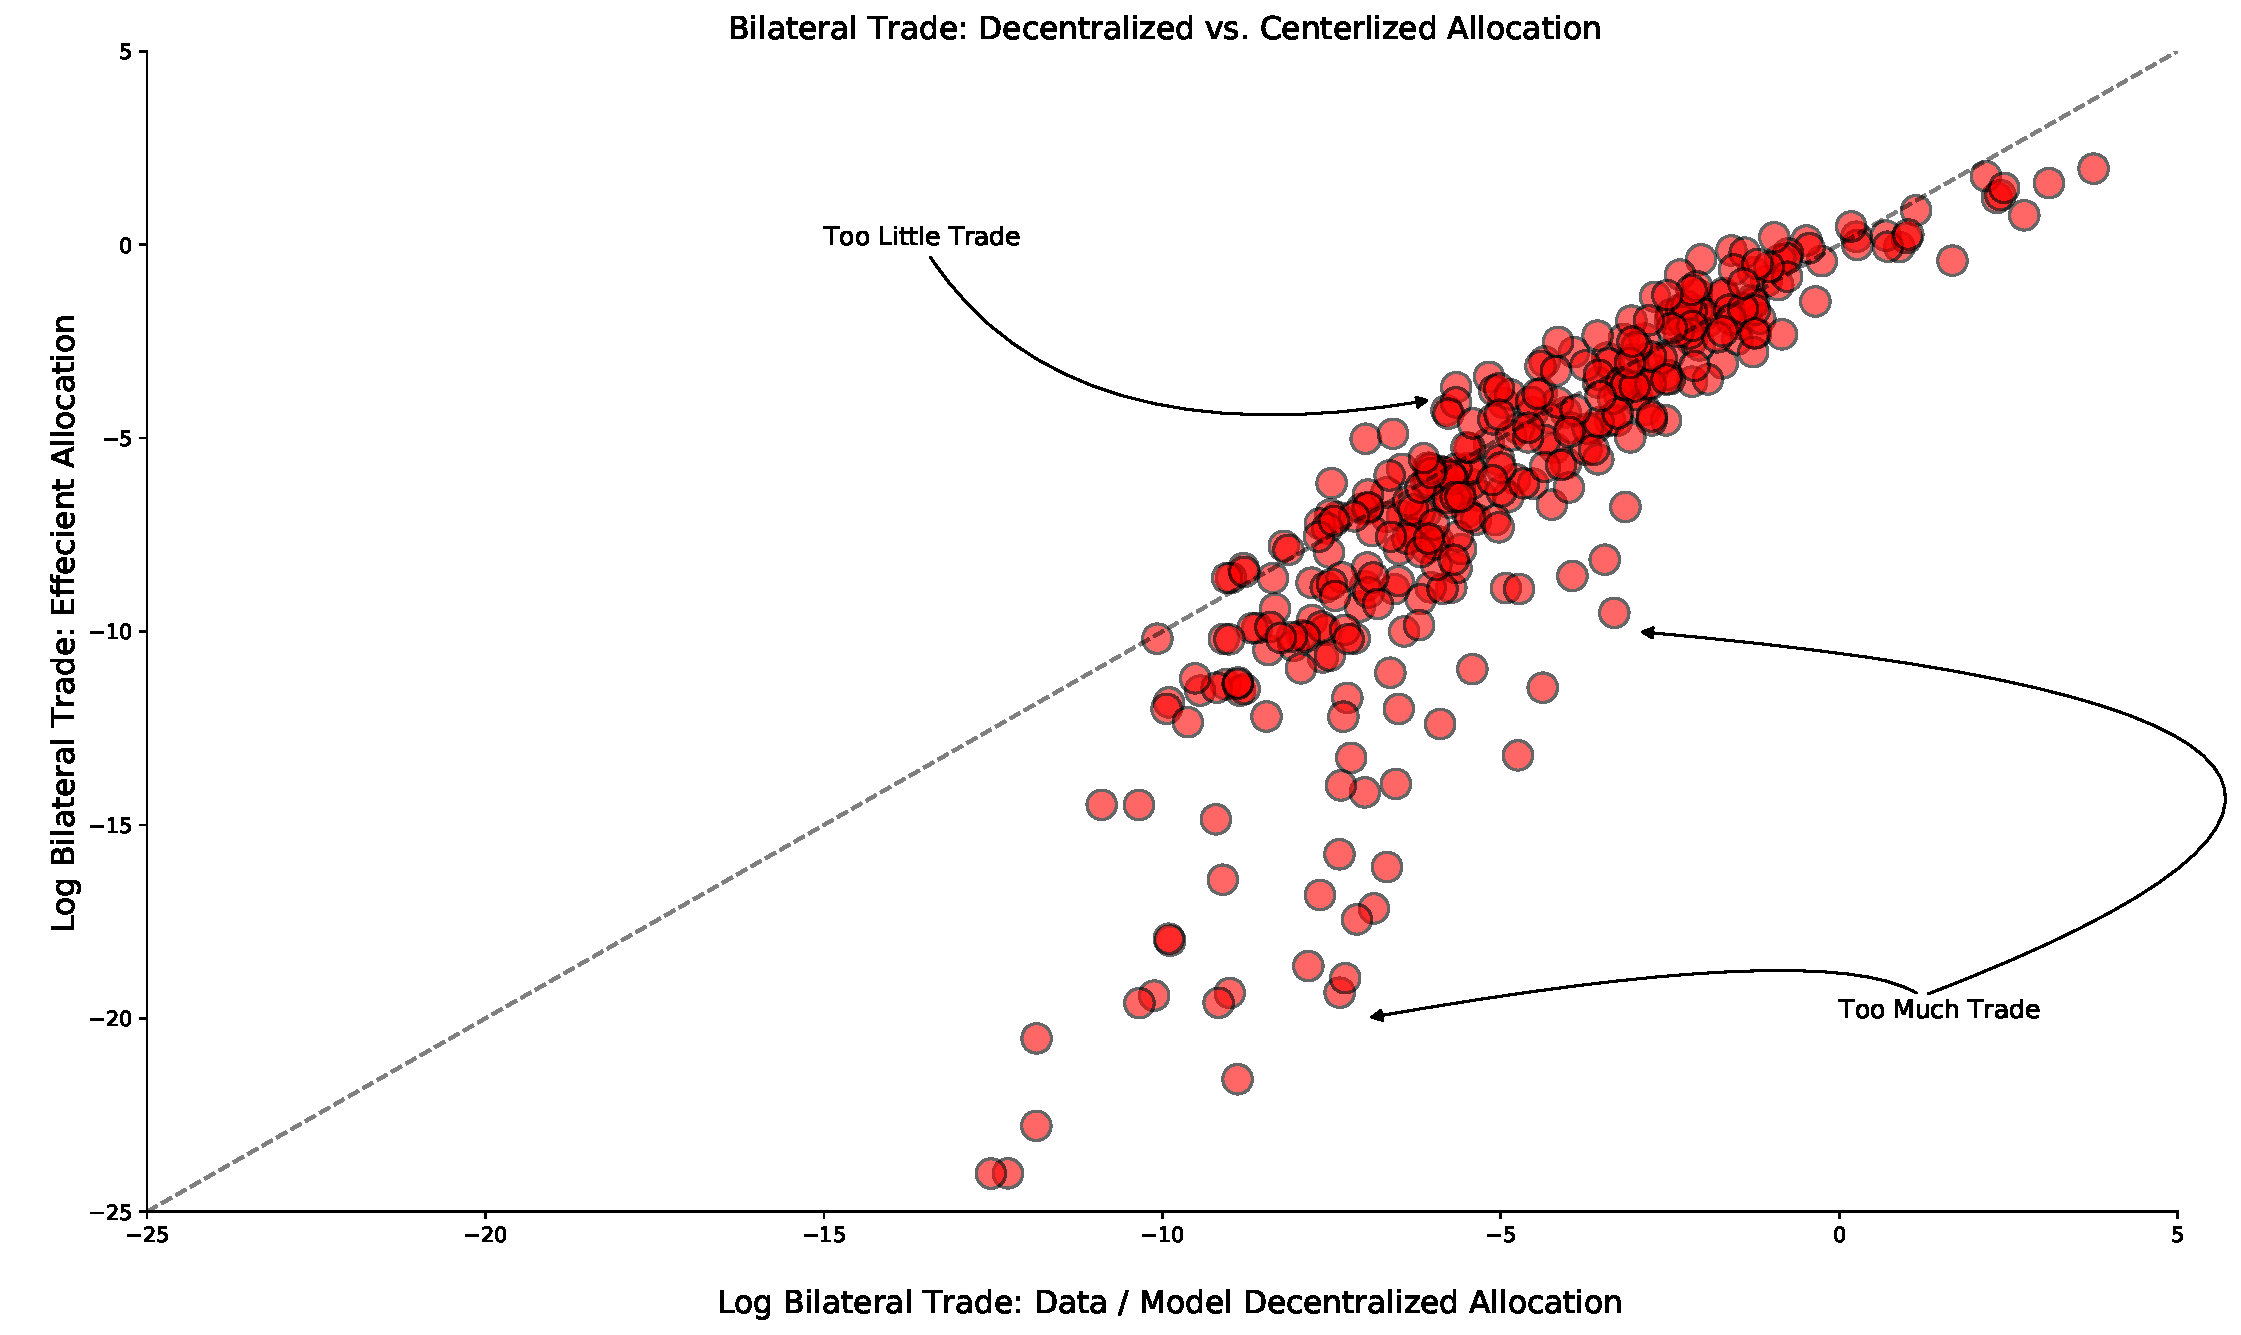
\includegraphics[scale = .35]{../notes/figures/decentralized-trade-all.pdf}}
\end{figure}

\end{frame}

\begin{frame}[t]{US Imports: Decentralized vs. Efficient Allocation}

\begin{figure}[!t]
\begin{subfigure}{}
    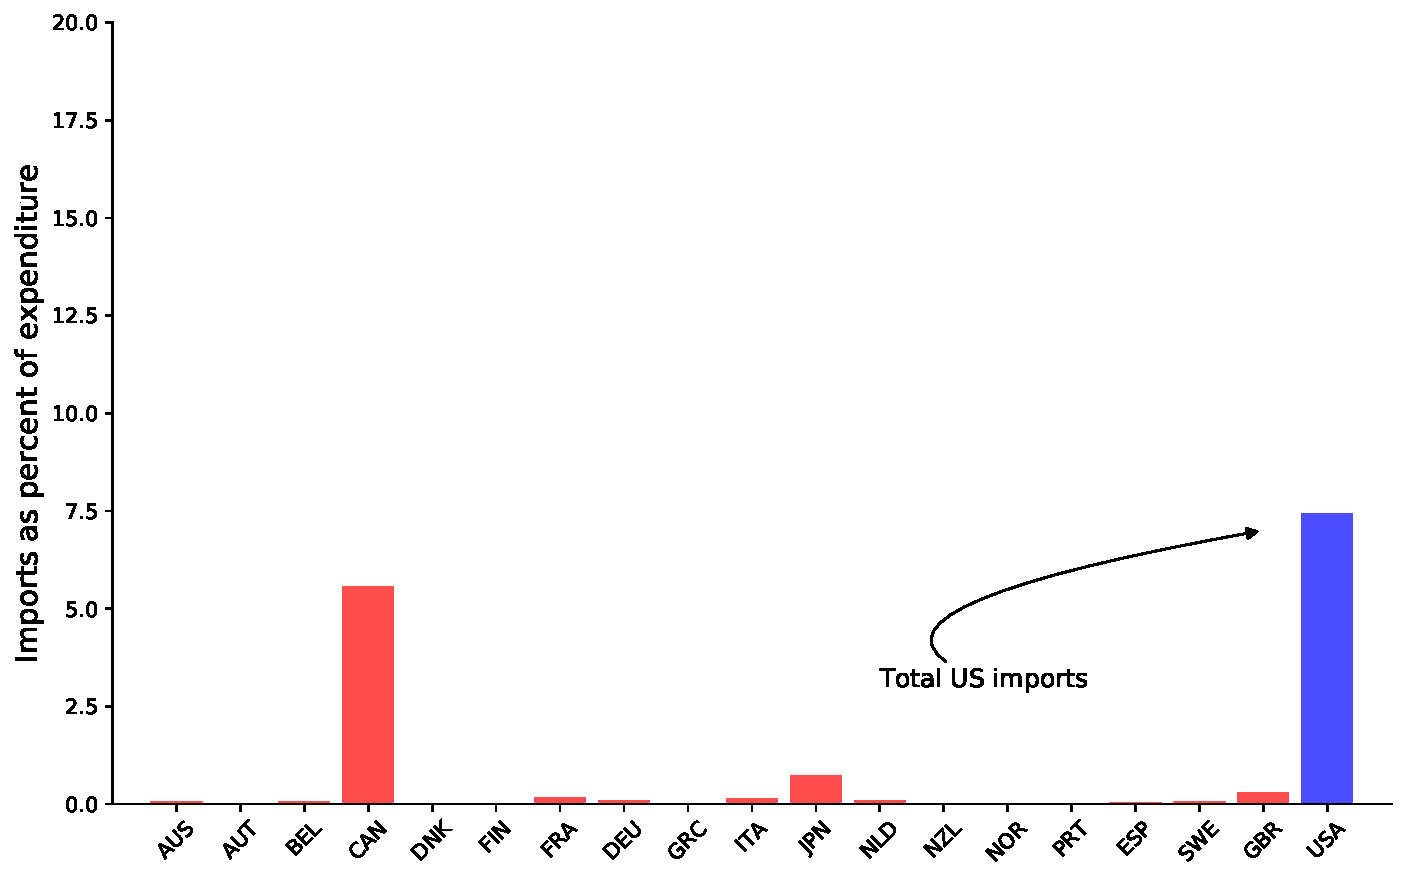
\includegraphics[scale = 0.26]{../notes/figures/decentralized-trade-us.pdf}
\end{subfigure}
\begin{subfigure}{}
    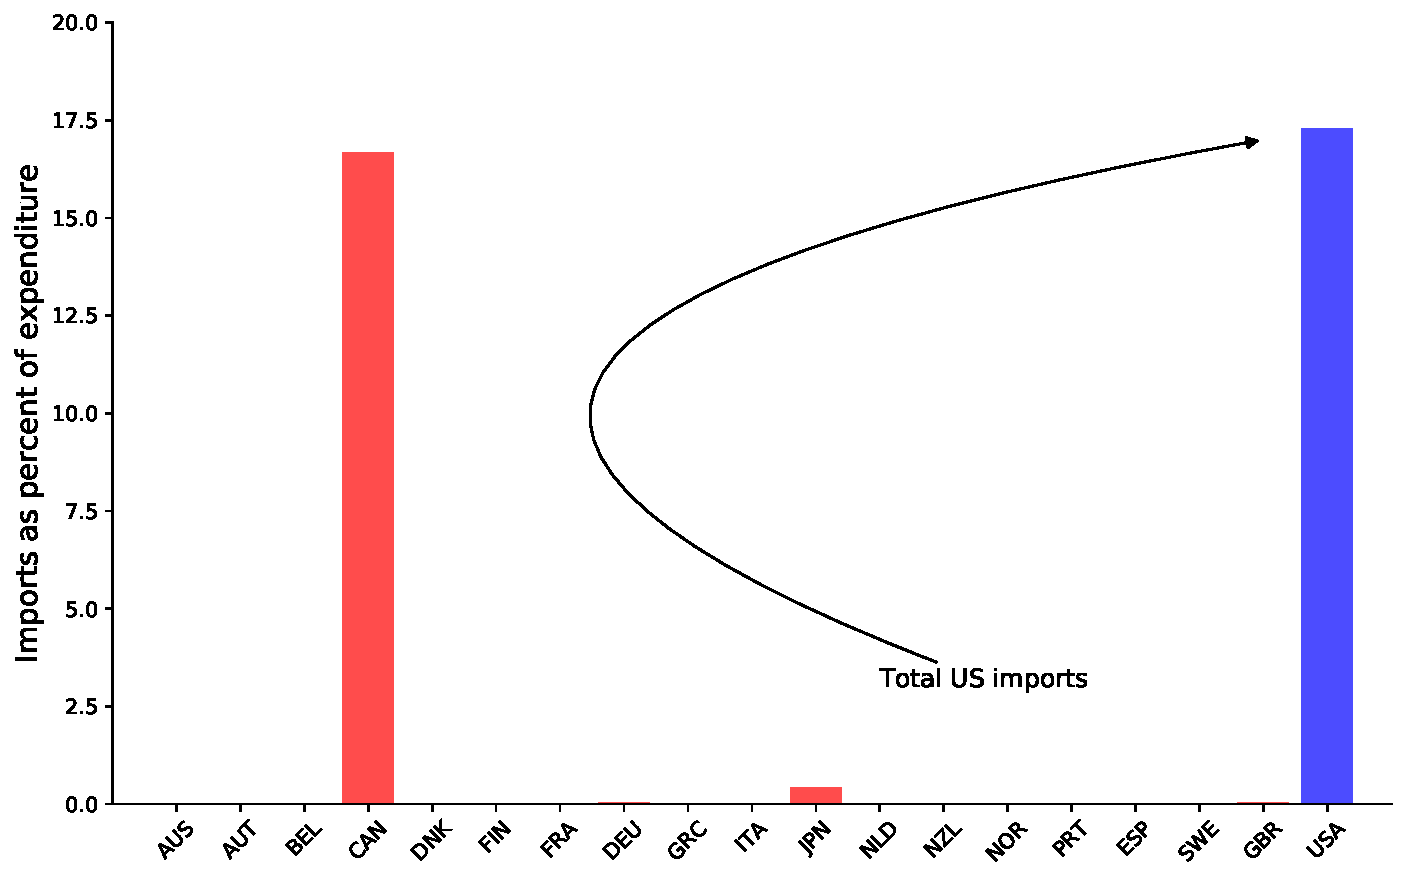
\includegraphics[scale = 0.26]{../notes/figures/planner-trade-us.pdf}
\end{subfigure}
\end{figure}
\bigskip
For the US, the Planner reallocates trade and expands it\ldots
\begin{itemize}
\smallskip
\item Squashes trade with uncompetitive sources | these varieties are like luxuries in that they only cater to the rich like France.
\smallskip
\item Expands trade with sources that can ``serve the masses'' like Japan (productive and large).
\smallskip
\item On net, US trade expands\ldots but this does not happen everywhere.
\end{itemize}
\end{frame}

%%%%%%%%%%%%%%%%%%%%%%%%%%%%%%%%%%%%%%%%%%%%%%%%%%%%%%%%%%%%%%%%%%%%%%%%%%%%%%%%%%%%%%%%%%%%%%%%
%%%%%%%%%%%%%%%%%%%%%%%%%%%%%%%%%%%%%%%%%%%%%%%%%%%%%%%%%%%%%%%%%%%%%%%%%%%%%%%%%%%%%%%%%%%%%%%%

\begin{frame}[t]
\frametitle{Where I'm headed next\ldots}
\smallskip
On my todo list:
\begin{itemize}
\smallskip
\item Can trade policy improve outcomes? Put in tariffs and redistribute.
\smallskip
\item Quality or ``residual demand shifters'' and calibration to line up with the micro-evidence of papers like \citet{auer2022unequal}.
\end{itemize}
\medskip
Any thing else? Email me!\\
\bigskip
One more thing: My github repository provides the code and supplementary work behind this paper at \url{https://github.com/mwaugh0328/heterogeneous-agent-trade}.

\end{frame}

%%%%%%%%%%%%%%%%%%%%%%%%%%%%%%%%%%%%%%%%%%%%%%%%%%%%%%%%%%%%%%%%%%%%%%%%%%%%%%%%%%%%%%%%%%%%%%%%
%%%%%%%%%%%%%%%%%%%%%%%%%%%%%%%%%%%%%%%%%%%%%%%%%%%%%%%%%%%%%%%%%%%%%%%%%%%%%%%%%%%%%%%%%%%%%%%%

%%%%%%%%%%%%%%%%%%%%%%%%%%%%%%%%%%%%%%%%%%%%%%%%%%%%%%%%%%%%%%%%%%%%%%%%%%%%%%%%%%%%%%%%%%%%%%%%
%%%%%%%%%%%%%%%%%%%%%%%%%%%%%%%%%%%%%%%%%%%%%%%%%%%%%%%%%%%%%%%%%%%%%%%%%%%%%%%%%%%%%%%%%%%%%%%%

\appendix

\newcounter{finalframe}
\setcounter{finalframe}{\value{framenumber}}

\begin{frame}[allowframebreaks]
\frametitle{References}
\scriptsize
\bibliography{../notes/bibtex/micro_price_bibtex}
\end{frame}


\begin{frame}[t]{Log Model | Fit of Trade Data}
\begin{figure}[!t]
\centering{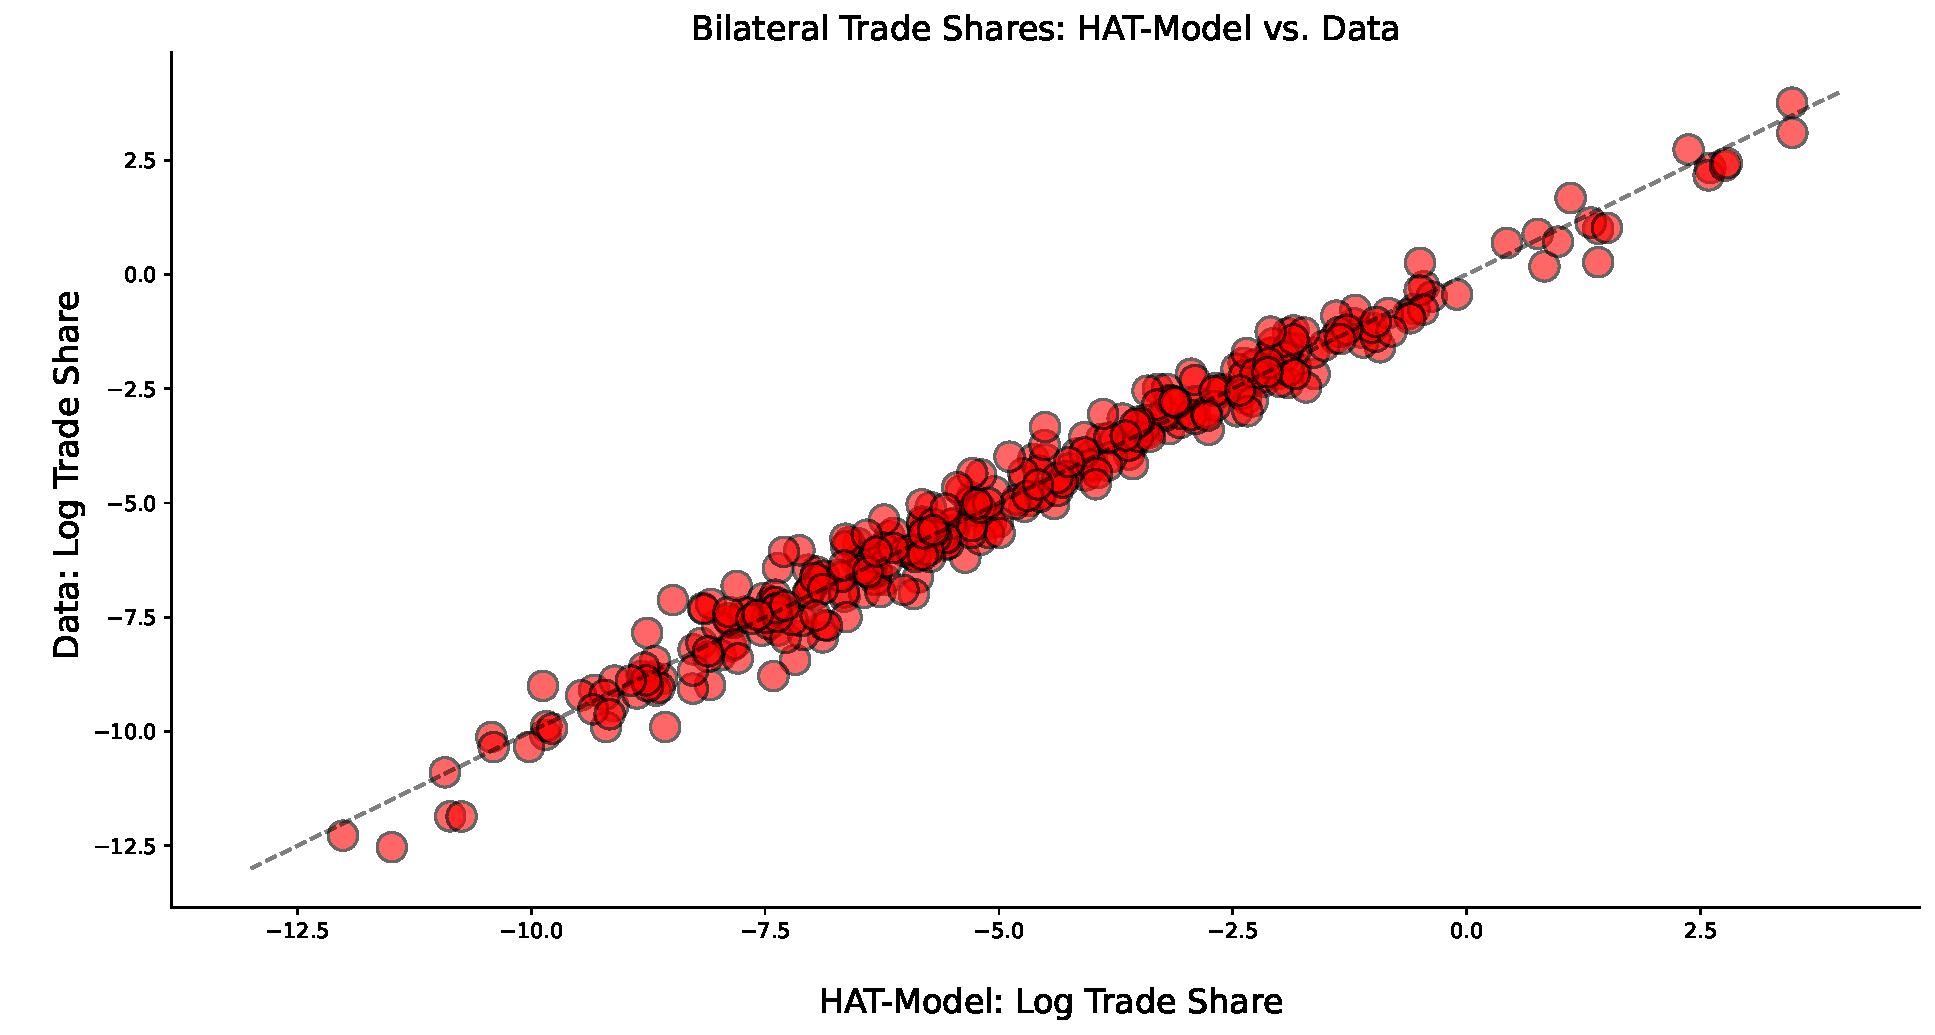
\includegraphics[scale = .35]{../notes/figures/log-trade-fit.pdf}}
\end{figure}
\end{frame}

\begin{frame}[t]{Log Model | Micro Elasticities}
\begin{figure}[!t]
\centering{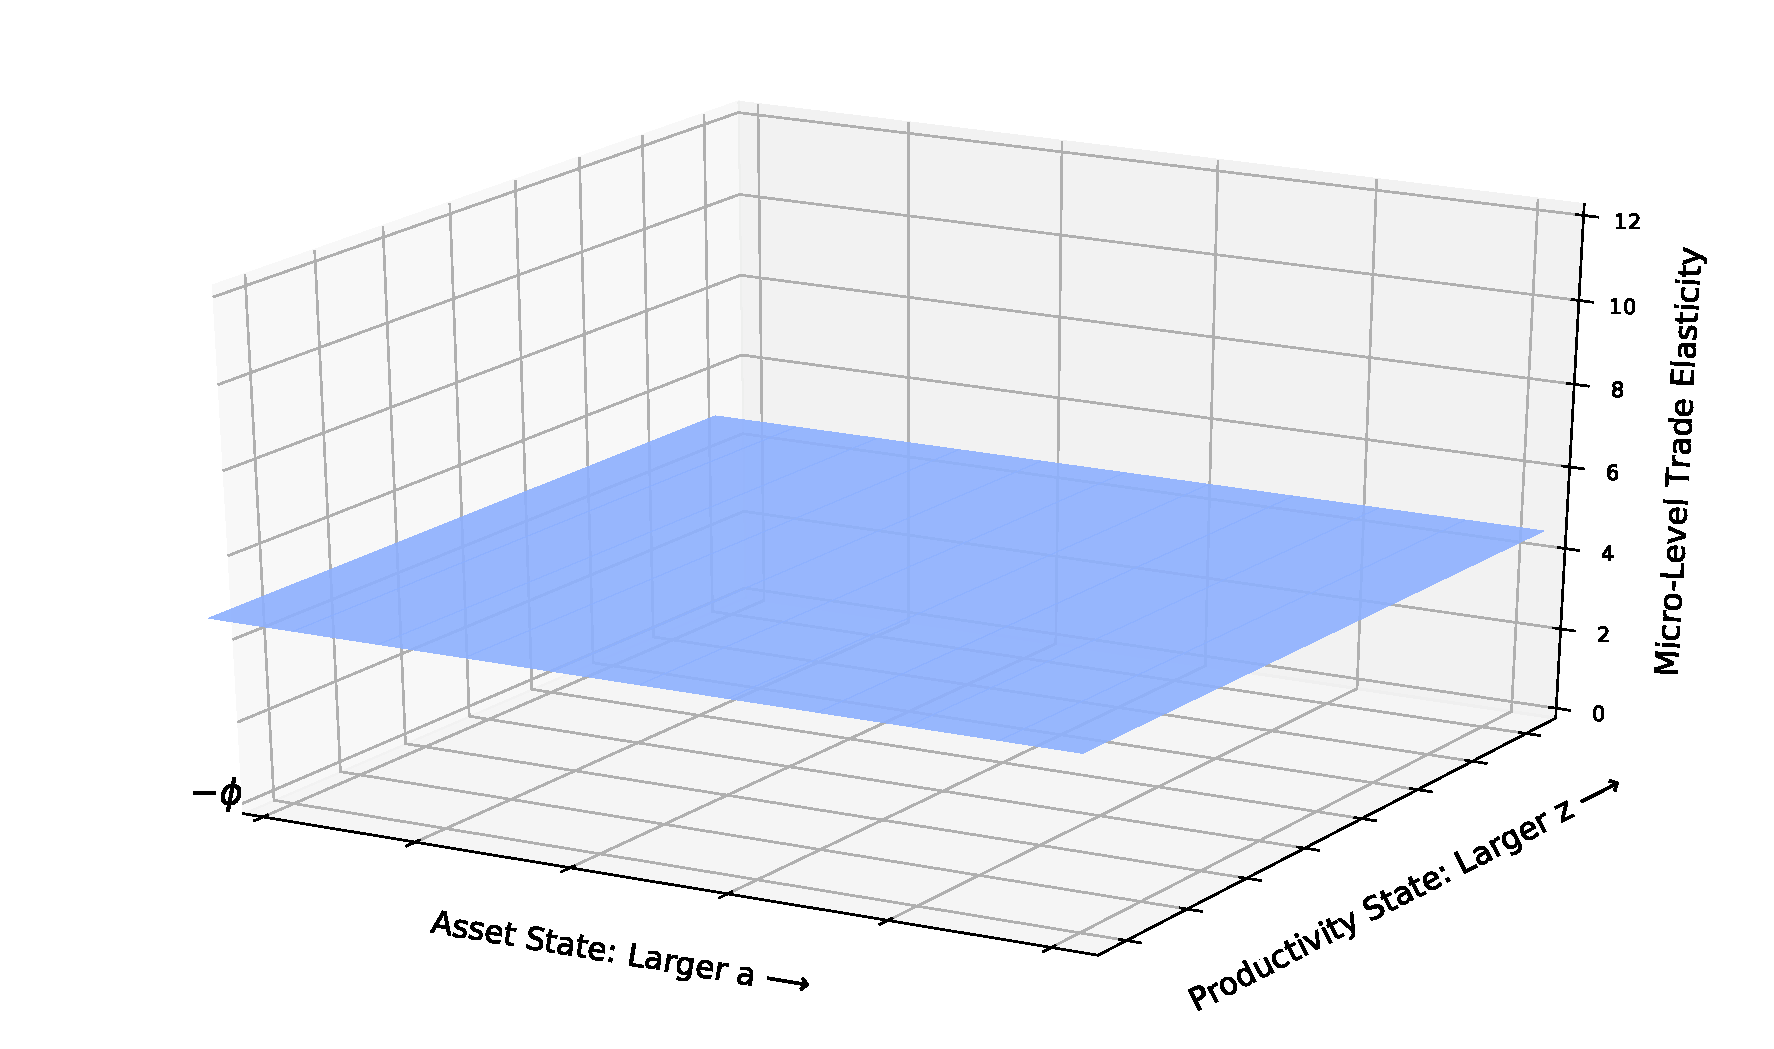
\includegraphics[scale = .4]{../notes/figures/micro-elasticity-log.pdf}}
\end{figure}
\end{frame}


%%%%%%%%%%%%%%%%%%%%%%%%%%%%%%%%%%%%%%%%%%%%%%%%%%%%%%%%%%%%%%%%%%%%%%%%%%%%%%%%%%%%%%%%%%%%%%%%%
%%%%%%%%%%%%%%%%%%%%%%%%%%%%%%%%%%%%%%%%%%%%%%%%%%%%%%%%%%%%%%%%%%%%%%%%%%%%%%%%%%%%%%%%%%%%%%%%%

\begin{frame}[t]{Micro-Elasticities I: The Intensive Margin}
\smallskip
How do households respond on the \textbf{intensive} margin to a change in trade costs?
\begin{align*}
\theta_{ij}(a,z)^{I} & := \frac{\partial c_{ij}(a,z)/ c_{ij}(a,z)}{\partial d_{ij} / d_{ij}}, \\
\\
& = \bigg [-\frac{\partial g_{ij}(a,z)/ p_{ij}c_{ij}(a,z)}{\partial p_{ij}/ p_{ij}} - 1 \bigg ]\frac{\partial p_{ij}/p_{ij}}{\partial d_{ij}/ d_{ij}}.
\end{align*}\\
\bigskip
\medskip
The idea: A reduction in trade costs relaxes the hh's budget constraint, so the intensive margin elasticity depends on the division of new resources between assets and expenditure.
\end{frame}

%%%%%%%%%%%%%%%%%%%%%%%%%%%%%%%%%%%%%%%%%%%%%%%%%%%%%%%%%%%%%%%%%%%%%%%%%%%%%%%%%%%%%%%%%%%%%%%%
%%%%%%%%%%%%%%%%%%%%%%%%%%%%%%%%%%%%%%%%%%%%%%%%%%%%%%%%%%%%%%%%%%%%%%%%%%%%%%%%%%%%%%%%%%%%%%%%

\begin{frame}[t]{Micro-Elasticities II: The Extensive Margin}
\smallskip
How do households respond on the \textbf{extensive} margin?
\begin{align*}
\theta_{ij}(a,z)^{E} &:= \frac{\partial \pi_{ij}(a,z) / \pi_{ij}(a,z)}{\partial d_{ij} / d_{ij}}, \\
\nonumber \\
& = - \frac{\partial \Phi_{i}(a,z) / \Phi_{i}(a,z)}{\partial d_{ij}/d_{ij}} -\frac{1}{\sigma_{\epsilon}}\bigg[u'(c_{ij}(a,z))c_{ij}(a,z)\bigg] + \beta \mathbb{E}\frac{1}{\sigma_{\epsilon}}\frac{\partial v_{i}(a',z')}{\partial d_{ij}/ d_{ij}}.
\end{align*}\\
\medskip
\bigskip
\uncover<2>{To get a sense of things, vary the second term by wealth\ldots
\begin{align*}
\frac{\partial (u'(c_{ij}(a,z))c_{ij}(a,z))}{\partial a} = u'(c_{ij}(a,z))\times \mathbf{MPC}_{ij}(a,z) \times \bigg[-\rho_{ij}(a,z) + 1\bigg],
\end{align*}\\
\medskip
where $\rho_{ij}(a,z)$ is the Arrow-Pratt measure of relative risk aversion.\\
\medskip
With CRRA, if risk aversion $> \ 1 \ $, then poor, high marginal utility households (who are also high MPC households) are \emph{more elastic relative} to rich households on the extensive margin.}
\end{frame}

%%%%%%%%%%%%%%%%%%%%%%%%%%%%%%%%%%%%%%%%%%%%%%%%%%%%%%%%%%%%%%%%%%%%%%%%%%%%%%%%%%%%%%%%%%%%%%%%
%%%%%%%%%%%%%%%%%%%%%%%%%%%%%%%%%%%%%%%%%%%%%%%%%%%%%%%%%%%%%%%%%%%%%%%%%%%%%%%%%%%%%%%%%%%%%%%%


\setcounter{framenumber}{\value{finalframe}}

%%%%%%%%%%%%%%%%%%%%%%%%%%%%%%%%%%%%%%%%%%%%%%%%%%%%%%%%%%%%%%%%%%%%%%%%%%%%%%%%%%%%%%%%%%%%%%%%%
%%%%%%%%%%%%%%%%%%%%%%%%%%%%%%%%%%%%%%%%%%%%%%%%%%%%%%%%%%%%%%%%%%%%%%%%%%%%%%%%%%%%%%%%%%%%%%%%%



\end{document} 